%%%%%%%%%%%%%%%%%%%%%%%%%%%%%%%%%%%%%%%%%
% Beamer Presentation
% LaTeX Template
% Version 1.0 (10/11/12)
%
% This template has been downloaded from:
% http://www.LaTeXTemplates.com
%
% License:
% CC BY-NC-SA 3.0 (http://creativecommons.org/licenses/by-nc-sa/3.0/)
%
%%%%%%%%%%%%%%%%%%%%%%%%%%%%%%%%%%%%%%%%%
%----------------------------------------------------------------------------------------
%	PACKAGES AND THEMES
%----------------------------------------------------------------------------------------
% Interessante: 
%https://www.codecogs.com/latex/eqneditor.php?lang=pt-br


\documentclass{beamer}

\usepackage[brazilian]{babel}
\usepackage[utf8]{inputenc}
\usepackage[T1]{fontenc}
\usepackage{colortbl}
\usepackage{mathrsfs}
\usepackage{smartdiagram}
\usepackage{listings}
\usepackage[framed,numbered,autolinebreaks,useliterate]{mcode}
\usepackage{multirow}
\usepackage{amssymb}
\usepackage{mdframed}
\usepackage{listings}
\usepackage{amsmath}
\usepackage[framed,numbered,autolinebreaks,useliterate]{mcode}



\mode<presentation> {

% The Beamer class comes with a number of default slide themes
% which change the colors and layouts of slides. Below this is a list
% of all the themes, uncomment each in turn to see what they look like.

%\usetheme{default}
%\usetheme{AnnArbor}
%\usetheme{Antibes}
%\usetheme{Bergen}
%\usetheme{Berkeley}
%\usetheme{Berlin}
%\usetheme{Boadilla}
%\usetheme{CambridgeUS}
%\usetheme{Copenhagen}
%\usetheme{Darmstadt}
%\usetheme{Dresden}
\usetheme{Frankfurt}
%\usetheme{Goettingen}
%\usetheme{Hannover}
%\usetheme{Ilmenau}
%\usetheme{JuanLesPins}
%\usetheme{Luebeck}
%\usetheme{Madrid}
%\usetheme{Malmoe}
%\usetheme{Marburg}
%\usetheme{Montpellier}
%\usetheme{PaloAlto}
%\usetheme{Pittsburgh}
%\usetheme{Rochester}
%\usetheme{Singapore}
%\usetheme{Szeged}
%\usetheme{Warsaw}

% As well as themes, the Beamer class has a number of color themes
% for any slide theme. Uncomment each of these in turn to see how it
% changes the colors of your current slide theme.

%\usecolortheme{albatross}
%\usecolortheme{beaver}
%\usecolortheme{beetle}
%\usecolortheme{crane}
%\usecolortheme{dolphin}
%\usecolortheme{dove}
%\usecolortheme{fly}
%\usecolortheme{lily}
%\usecolortheme{orchid}
%\usecolortheme{rose}
%\usecolortheme{seagull}
%\usecolortheme{seahorse}
%\usecolortheme{whale}
%\usecolortheme{wolverine}

%\setbeamertemplate{footline} % To remove the footer line in all slides uncomment this line
%\setbeamertemplate{footline}[page number] % To replace the footer line in all slides with a simple slide count uncomment this line

%\setbeamertemplate{navigation symbols}{} % To remove the navigation symbols from the bottom of all slides uncomment this line
}

\usepackage{graphicx} % Allows including images
\usepackage{booktabs} % Allows the use of \toprule, \midrule and \bottomrule in tables

\usepackage{animate}
\usepackage{hyperref}
\usepackage{media9}
\usepackage{listings}
\usepackage{amsmath}
\usepackage[framed,numbered,autolinebreaks,useliterate]{mcode}
\usepackage{chronology}
\usepackage{xpatch}
\xpretocmd{\chronology}{\tikzset{>=|}}{}{\failure}
\usepackage{mdframed}
\usepackage{tikz}
\usepackage{makecell}
\usetikzlibrary{arrows.meta}
\tikzset{%
  >={Latex[width=2mm,length=2mm]},
  % Specifications for style of nodes:
         base/.style = {rectangle, rounded corners, draw=black,
                        minimum width=4cm, minimum height=0.7cm,
                        text centered, font=\sffamily},
         activityStarts/.style = {base, fill=blue!30},
         process/.style = {base, minimum width=2.5cm, fill=orange!15,
                          font=\ttfamily},
         ilumina/.style = {base, minimum width=2.5cm, fill=red!55,
                          font=\ttfamily},           
         coord/.style={coordinate, on chain, on grid, node distance=6mm and 25mm},
}

\usetikzlibrary{arrows,shapes,positioning,shadows,trees}

\tikzset{
  basic/.style  = {draw, text width=2cm, drop shadow, font=\sffamily, rectangle},
  root/.style   = {basic, rounded corners=2pt, thin, align=center,
                   fill=green!30},
  level 2/.style = {basic, rounded corners=6pt, thin,align=center, fill=green!60,
                   text width=8em},
  level 3/.style = {basic, thin, align=left, fill=pink!60, text width=6.5em}
}

%----------------------------------------------------------------------------------------
%	TITLE PAGE
%----------------------------------------------------------------------------------------

\logo
{
    
\includegraphics[width=0.6cm,height=0.6cm,keepaspectratio]{UFJF.jpg}~%
}

\title[Aula 2]{Programação Linear} 

\author
{
Prof. André Luís Marques Marcato \\
%\small andre.marcato@ufjf.edu.br
\href{mailto:andre.marcato@ufjf.edu.br}{\beamergotobutton{ andre.marcato@ufjf.edu.br }}
} % Your name

\institute[UFJF] % Your institution as it will appear on the bottom of every slide, may be shorthand to save space
{
Universidade Federal de Juiz de Fora \\

\includegraphics[width=1cm]{Engenharia.jpg} \\
}

%\date{\small \today} % Date, can be changed to a custom date
\date{\small Primeiro Semestre de 2018} % Date, can be changed to a custom date

\hypersetup{
    colorlinks=true,
    linkcolor=gray,
    filecolor=magenta,      
    urlcolor=cyan,
}

\begin{document}

\begin{frame}
\titlepage % Print the title page as the first slide
\begin{figure}[!htb]
\centering
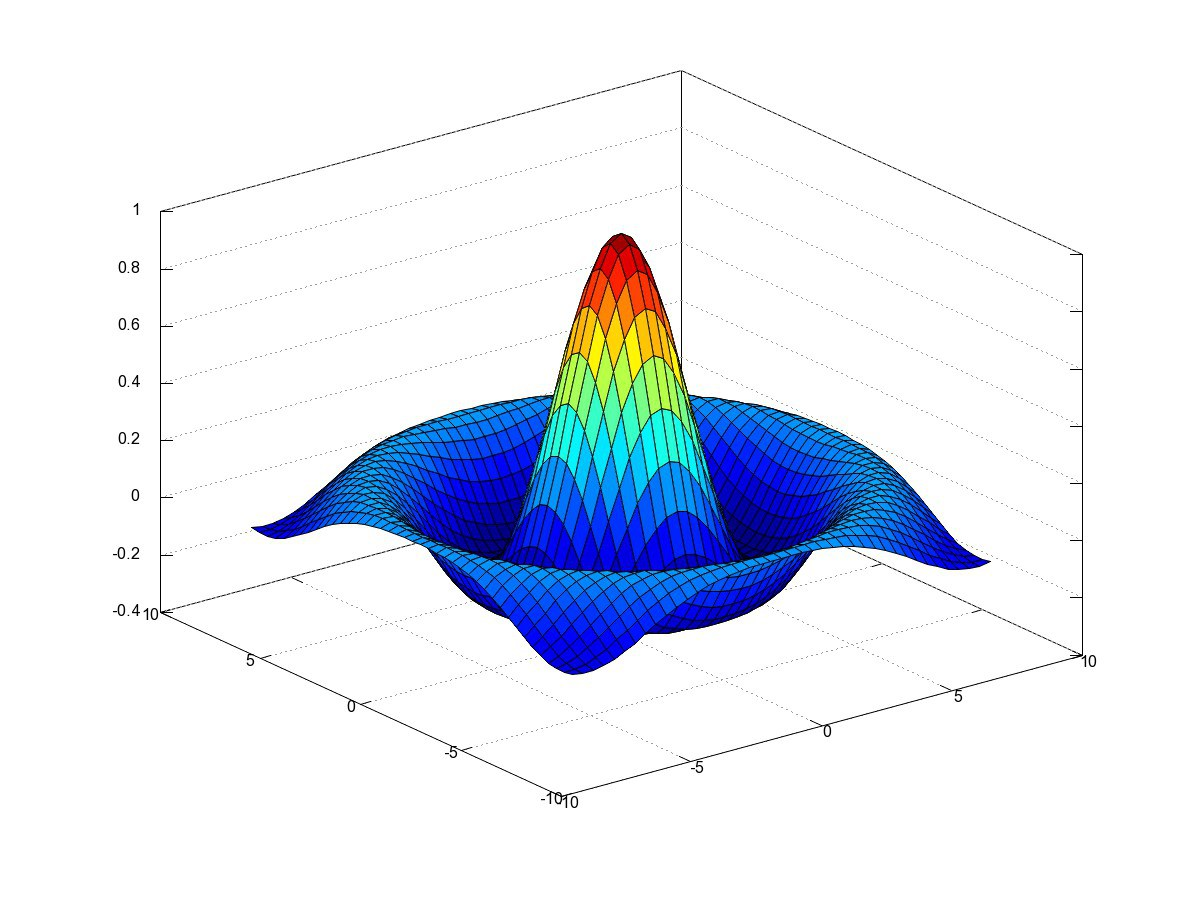
\includegraphics[width=2.6cm, height=1.7cm]{cover.jpg}
%\caption{Ogata - 5a Edicao - Fig. 1.1}
\label{Ogata_1_1}
\end{figure}
\end{frame}

\begin{frame}
\frametitle{Agenda da Apresentação} % Table of contents slide, comment this block out to remove it
\tableofcontents % Throughout your presentation, if you choose to use \section{} and \subsection{} commands, these will automatically be printed on this slide as an overview of your presentation
\end{frame}

%----------------------------------------------------------------------------------------
%	PRESENTATION SLIDES
%----------------------------------------------------------------------------------------

%\include{intro_e_avanco}

\section{Introdução}
\subsection{Histórico}

\begin{frame}
\frametitle{Histórico}
\centering
\begin{table}
	\begin{tabular}{c c}
	\only<1>{
				\multirow{5}{*}{\includegraphics[width=3cm,height=3cm]{fourier.jpg}} &
								Jean Baptiste Joseph Fourier (matemático \\ 
							  & Francês). Ele publicou um trabalho sobre a \\
							  & resolução de sistemas de equações lineares. \\
							  & Este trabalho é considerado o primeiro sobre \\
							  & programação linear. \\ 
				\multicolumn{2}{c}
				{
					\begin{chronology}[20]{1820}{2020}{\textwidth}
						\small
						\event{1827}{ {\color{red} 1827} - Fourier}
					\end{chronology} 
				} \\
			}
	\only<2>{
				\multirow{5}{*}{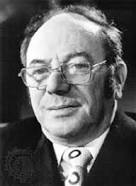
\includegraphics[width=3cm,height=3cm]{kantorovich.jpg}} &
								Leonide Kantorovich (matemático e economista \\ 
							  & Russo). Formulou e resolveu um problema de \\
							  & programação linear, mas seu trabalho permane- \\
							  & ceu desconhecido até 1959. \\
							  &  \\ 
				\multicolumn{2}{c}
				{
				\begin{chronology}[20]{1820}{2020}{\textwidth}
					\small
					\event[1939]{1959}{ {\color{red} 1939} - Kantorovich}
				\end{chronology} 
				} \\
			}
	\only<3>{
				\multirow{5}{*}{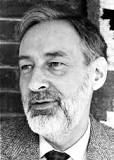
\includegraphics[width=3cm,height=3cm]{koopmans.jpg}} &
								O termo \alert{\underline{programação linear}} foi criado pelo   \\
							  & economista Holandês Tjalling Koopmans em \\
							  & uma conversa com Datzig na California  \\
							  & em 1948. Ele formulou modelos de progra- \\
							  & ção linear aplicados em economia clássica. \\ 
				\multicolumn{2}{c}
				{
				\begin{chronology}[20]{1820}{2020}{\textwidth}
					\small
					\event{1939}{ {\color{red} 1939} - Koopmans}
				\end{chronology} 
				} \\
			}
	\only<4>{
				\multirow{5}{*}{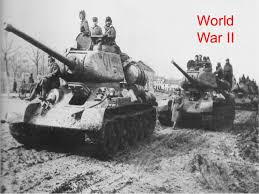
\includegraphics[width=3cm,height=3cm]{secondwar.jpg}} &
								Durante a Segunda Guerra Mundial, mode- \\
							  & los de programação linear foram  projetados \\
							  & e resolvidos em aplicações voltadas para  \\
							  & planejamento militar. \\
							  &  \\ 
				\multicolumn{2}{c}
				{
				\begin{chronology}[20]{1820}{2020}{\textwidth}
					\small
					\event[1939]{1945}{ {\color{red} Second War}}
				\end{chronology} 
				} \\
			}
	\only<5>{
				\multirow{5}{*}{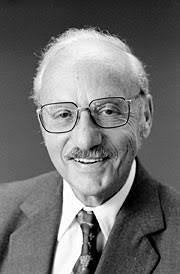
\includegraphics[width=3cm,height=3cm]{dantzig.jpg}} &
								Em 1947, George Dantzig desenvolveu o \\
							  & \alert{\underline{Método Simplex}}, propondo a Formulação \\ 
							  & Geral de Problemas de Programação Linear.  \\ 
							  & Ele trabalhava como  matemático consultor   \\
							  & para o Pentágono.\\ 
				\multicolumn{2}{c}
				{
				\begin{chronology}[20]{1820}{2020}{\textwidth}
					\small
					\event[1939]{1947}{ {\color{red} 1947} - Dantzig}
				\end{chronology} 
				} \\
			}			
	\only<6>{
				\multirow{5}{*}{
\includegraphics[width=3cm,height=3cm]{nobel.jpg}} &
								Em 1975, Kantorovich e Koopmans receberam   \\
							  & o Prêmio Nobel em Ciências Econômicas pelo \\
							  & trabalho desenvolvido na área de programação \\
							  & linear. \\
							  &  \\ 
				\multicolumn{2}{c}
				{
				\begin{chronology}[20]{1820}{2020}{\textwidth}
					\small
					\event{1975}{ {\color{red} 1975} - Prêmio Nobel}
				\end{chronology} 
				} \\
			}
	\only<7>{
				\multirow{5}{*}{
\includegraphics[width=3cm,height=3cm]{bitcoin.jpg}} &
								Atualmente, problemas de prog. linear   \\
							  & são resolvidos 1.000.000 de vezes mais \\
							  & rapidamente que 1985. Além disto, problemas  \\
							  & com mais de 1.000.000 variáveis e restrições \\
							  & são prontamente resolvidos.  \\ 
				\multicolumn{2}{c}
				{
				\begin{chronology}[20]{1820}{2020}{\textwidth}
					\small
					\event{2018}{ {\color{red} 2018} }
				\end{chronology} 
				} \\
			}			
\end{tabular}
\end{table}
\end{frame}

\begin{frame}
	\frametitle{Programação Linear - Histórico}
	\begin{itemize}
	\item[] {Os maiores problemas na resolução de PL na época}
		\begin{itemize}
		\only<1->
		{
		\item[] 
\includegraphics[width=0.5cm,height=0.2cm]{seta.png} Achar um ponto inicial, ponto de partida do algoritmo.
		} 
		\only<2->
		{
		\item[] 
\includegraphics[width=0.5cm,height=0.2cm]{seta.png} Reduzir a área de memória e o número de operações aritméticas sem causar limitações de uso.
		} 
		\only<3->
		{
		\item[] 
\includegraphics[width=0.5cm,height=0.2cm]{seta.png} Manter a precisão numérica para a obtenção de resultados significativos.
		} 
		\end{itemize}
	\only<4->
	{
	\item[] A partir de 1957, todos estes aspectos foram solucionados!
	} 
	\end{itemize}
\end{frame}

\subsection{Modelagem Matemática}

\begin{frame}
	\frametitle{Programação Linear - Modelagem Matemática}
	\begin{itemize}
	\item[] {Aspectos importantes para o levantamento do modelo:}
		\begin{itemize}
		\only<1->
		{
		\item[] 
\includegraphics[width=0.5cm,height=0.2cm]{seta.png} Identificação das variáveis;
		} 
		\only<2->
		{
		\item[] 
\includegraphics[width=0.5cm,height=0.2cm]{seta.png} Identificação dos objetivos.
		} 
		\only<3->
		{
		\item[] 
\includegraphics[width=0.5cm,height=0.2cm]{seta.png} Identificação dos aspectos restritivos.
		} 
		\end{itemize}
	\only<4->
	{
	\item[] O modelo é uma tentativa de representação da realidade e sua complexidade depende do grau de exatidão requerido.
	} 
	\end{itemize}
\end{frame}

\subsection{Exemplos}

\begin{frame}
	\frametitle{Programação Linear - Modelagem Matemática}
	\only<1>{
	\begin{columns}
		\begin{column}{0.7\textwidth}
			\centering
			\begin{exampleblock}{Exemplo 1}
				\scriptsize
				Um agricultor deseja cultivar duas variedades de cereais, \textbf{A} e \textbf{B}, em um área restrita a 100 ares ($100m^2$). Sendo que:
				\begin{itemize}
				\item 1 are do cereal \textbf{A} produz 8 sacas
				\item 1 are do cereal \textbf{B} produz 10 sacas
				\end{itemize}
				Para o plantio, cada cereal:
				\begin{itemize}
				\item Tipo \textbf{A} precisa de {\color{red} 3 homens-hora de trabalho por are}
				\item Tipo \textbf{B} precisa de {\color{red} 2 homens-hora de trabalho por are}
				\end{itemize}
				sendo que se dispõe até 240 homens-hora de trabalho para o cultivo e o custo da mão de obra é de \$200 (unidades monetárias) por homem-hora. \\~\\
				A demanda máxima é limitada pelo mercado a 480 sacas do cereal tipo \textbf{A}, vendido a \$150/saca, e 800 sacas do cereal \textbf{B}, vendido a \$120/saca. \\~\\
				O agricultor deseja otimizar a área de cultivo de forma a \alert{MAXIMIZAR O LUCRO}.
			\end{exampleblock}
		\end{column}
		\begin{column}{0.3\textwidth}
			\centering
			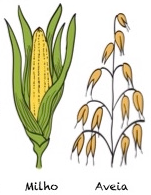
\includegraphics[width=2cm,height=3cm]{milho_aveia.png}
		\end{column}
	\end{columns}
	}
	\only<2>
	{
	\begin{columns}
		\begin{column}{0.7\textwidth}
			\centering
			\begin{exampleblock}{Exemplo 1 - As Variáveis do Problema}
				\scriptsize
				As variáveis estão relacionadas ao tamanho do terreno que será utilizado para o cultivo do cereal tipo \textbf{A} e \textbf{B}. Logo podemos definir;
				\begin{itemize}
				\item $x_1$: área destinada ao plantio do cereal Tipo \textbf{A}
				\item $x_2$: área destinada ao plantio do cereal Tipo \textbf{B} 
				\end{itemize}
			\end{exampleblock}
		\end{column}
		\begin{column}{0.3\textwidth}
			\centering
			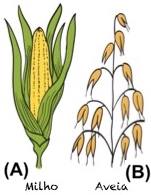
\includegraphics[width=2cm,height=3cm]{milho_aveia2.png}
		\end{column}
	\end{columns}	
	}	
	\only<3-7>
	{
	\begin{columns}
		\begin{column}{0.7\textwidth}
			\centering
			\begin{exampleblock}{Exemplo 1 - A Função Objetivo}
				\scriptsize
				Maximixar o lucro através da determinação ótima do tamanho do terreno que será utilizado para o cultivo dos cereais tipo \textbf{A} e \textbf{B}. \\~\\
				
				\begin{itemize}
				\item[]<4-> FOB = MAX LUCRO = MAX RECEITAS - CUSTOS
				\item<5-> $x_1$: Receitas: $receitas = \overset{\color{red}(150x8)}{1200}x_1+\overset{\color{red}(120x10)}{1200}x_2$
				\item<6-> $x_2$: Custos: $custos = \overset{\color{red}(200x3)}{600}x_1 + \overset{\color{red}(200x2)}{400}x_2$
				\item<7-> 
				$FOB = \max ({\color{red}600}x_1 + {\color{red}800}x_2)$ 
\includegraphics[width=1cm,height=1cm]{dinheiro2.jpg}
				\end{itemize}
			\end{exampleblock}
		\end{column}
		\begin{column}{0.3\textwidth}
			\centering
			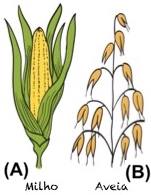
\includegraphics[width=2cm,height=3cm]{milho_aveia2.png}
		\end{column}
	\end{columns}	
	}
	\only<8-15>
	{
	\begin{columns}
		\begin{column}{0.7\textwidth}
			\centering
			\begin{exampleblock}{Exemplo 1 - As Restrições}
				\scriptsize
				\begin{itemize}
				\item<8-> {Desta forma a área custivada pelo cereal tipo \textbf{A} mais a área cultivada pelo cereal tipo \textbf{B} deve ocupar parte ou toda a área disponível de 100 ares}
					\begin{itemize}
					\item[$\circ$]<9->  $x_1+x_2 \le 100$
					\end{itemize}
				\item<10-> {Limitações de homem-hora}				
					\begin{itemize}
					\item[$\circ$]<11->  $3x_1+2x_2 \le 240$
					\end{itemize}
				\item<12-> {Limitações de devido à demanda de mercado}				
					\begin{itemize}
					\item[$\circ$]<13->  $8x_1 \le 480$ ou $x_1 \le 60$ para o cereal tipo \textbf{A}
					\item[$\circ$]<14->  $10x_2 \le 800$ ou $x_2 \le 80$ para o cereal tipo \textbf{B}
					\end{itemize}
				\end{itemize}
			\end{exampleblock}
		\end{column}
		\begin{column}{0.3\textwidth}
			\centering
			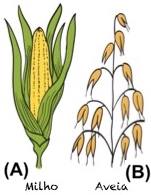
\includegraphics[width=2cm,height=3cm]{milho_aveia2.png}
		\end{column}
	\end{columns}
	}
	\only<16>
	{
	\begin{columns}
		\begin{column}{0.7\textwidth}
			\centering
			\begin{exampleblock}{Exemplo 1 - Modelo Matemático Completo}
				\scriptsize
				\begin{table}
					\begin{tabular}{r c l}
						$ \max Z = 600x_1+800x_2$ & 
\includegraphics[width=0.8cm,height=0.2cm]{seta2.png} & Função Objetivo \\
						sujeito a & & \\
						$x_1+x_2 \le 100$ & 
\includegraphics[width=0.8cm,height=0.2cm]{seta2.png}& Área Cultivo \\
						$3x_1+2x_2 \le 240$ & 
\includegraphics[width=0.8cm,height=0.2cm]{seta2.png}& Mão de Obra \\
						$x_1 \le 60 $ & 
\includegraphics[width=0.8cm,height=0.2cm]{seta2.png}& Produção Cereal \textbf{A} \\
						$x_2 \le 80 $ &
\includegraphics[width=0.8cm,height=0.2cm]{seta2.png} & Produção Cereal \textbf{B} \\
						$x_1, x_2 \ge 0$ & 
\includegraphics[width=0.8cm,height=0.2cm]{seta2.png}& Produção \\
					\end{tabular}
				\end{table}
			\end{exampleblock}
		\end{column}
		\begin{column}{0.3\textwidth}
			\centering
			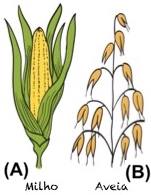
\includegraphics[width=2cm,height=3cm]{milho_aveia2.png}
		\end{column}
	\end{columns}	
	}
\end{frame}

\section{Solução Gráfica}
\subsection{Função Objetivo, Região Viável, Análise de Sensibilidade}

\begin{frame}
	\frametitle{Análise Gráfica} 
	\begin{columns}
		\begin{column}{0.5\textwidth}
			\centering
			\begin{exampleblock}{Exemplo 1 - Modelo Matemático}
				\scriptsize
				\begin{table}
					\begin{tabular}{r | l}
						{\color{red} $ \max Z = 600x_1+800x_2$ } & {\color{red} Objetivo } \\
						\only<10-24> 
						{
							sujeito a & \\
							{\color{blue}$x_1+x_2 \le 100$} &  {\color{blue} Área} \\
						}
						\only<12-24>
						{
							{\color{olive}$3x_1+2x_2 \le 240$} & {\color{olive}Mão de Obra} \\
						}
						\only<15-24>
						{
						{$x_1 \le 60 $ } & {Produção \textbf{A} } \\
						{$x_2 \le 80 $ } &  {Produção  \textbf{B} } \\
						{$x_1, x_2 \ge 0$ } &  {Produção } \\
						}
					\end{tabular}
				\end{table}
			\end{exampleblock}
			\only<22>
			{
		    \begin{mdframed}[backgroundcolor=pink] 
					A \underline{Região Viável} é a região de solução! É formada pelas restrições.
		    \end{mdframed}						
			}
			\only<23>
			{
		    \begin{mdframed}[backgroundcolor=pink] 
					A solução do problema estará na \underline{Região Viável}.
		    \end{mdframed}						
			}
			\only<24>
			{
			    \begin{mdframed}[backgroundcolor=blue!20] 
					Solução Ótima: $X_1 = 20$ e $X_2 = 80$ !!!
			    \end{mdframed}			
			}
		\end{column}
		\begin{column}{0.5\textwidth}
			\centering
			\only<1> {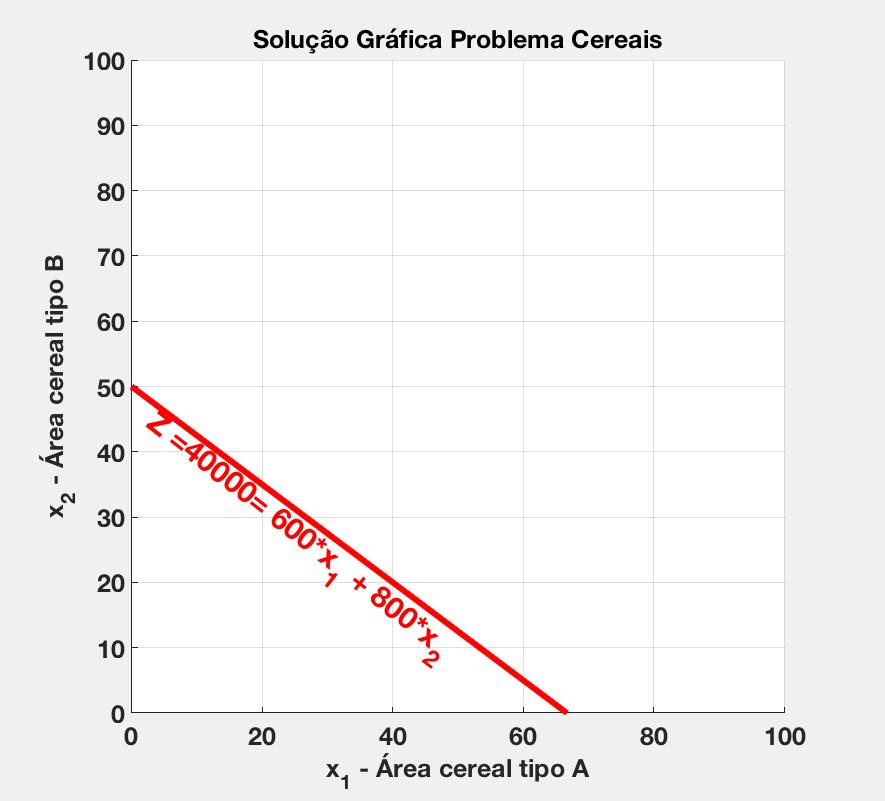
\includegraphics[width=6cm,height=6cm]{MatLab/anima_1.png} }
			\only<2> {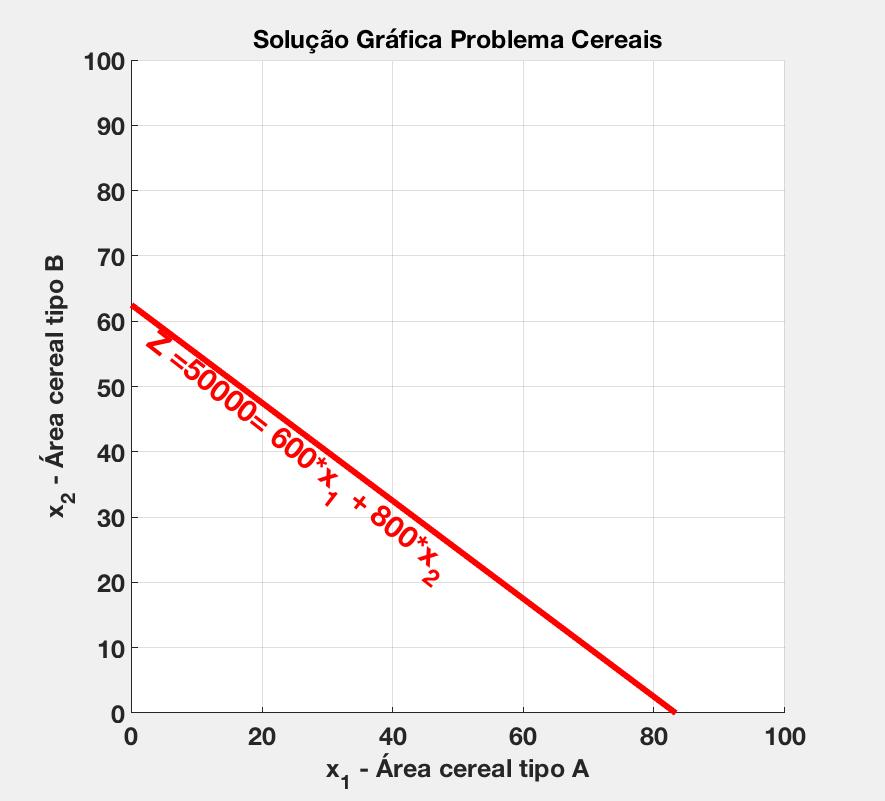
\includegraphics[width=6cm,height=6cm]{MatLab/anima_2.png} }
			\only<3> {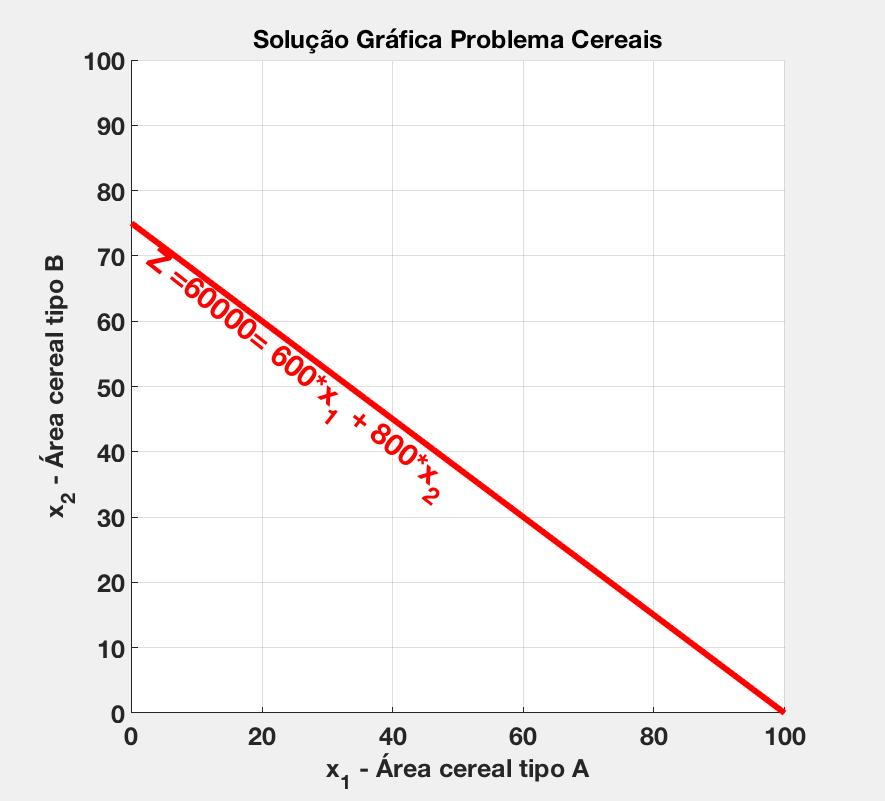
\includegraphics[width=6cm,height=6cm]{MatLab/anima_3.png} }
			\only<4> {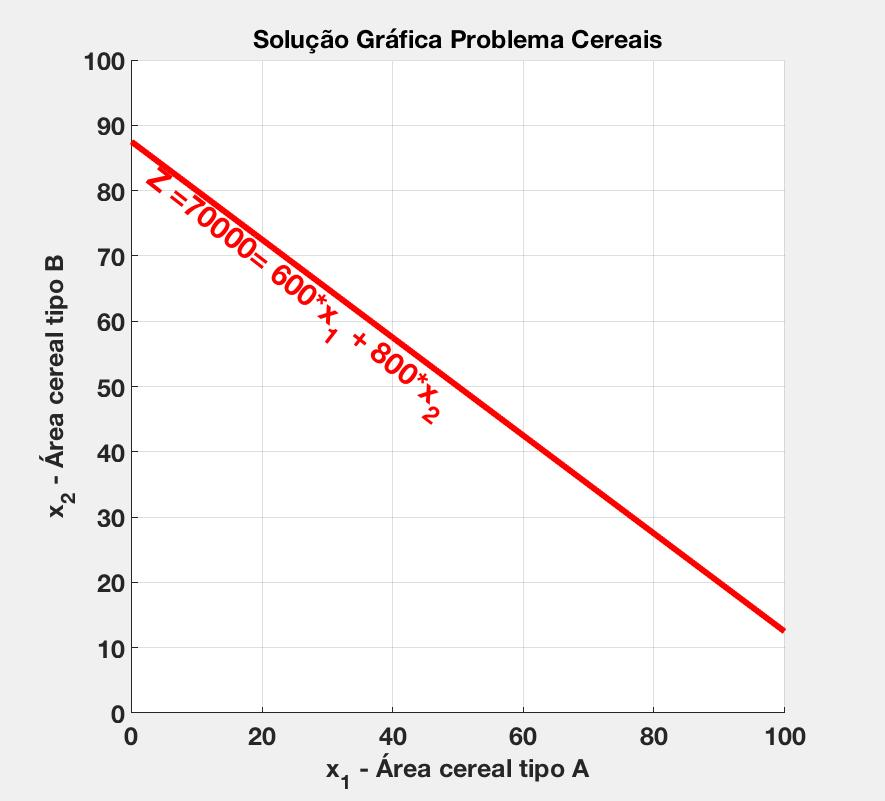
\includegraphics[width=6cm,height=6cm]{MatLab/anima_4.png} }
			\only<5> {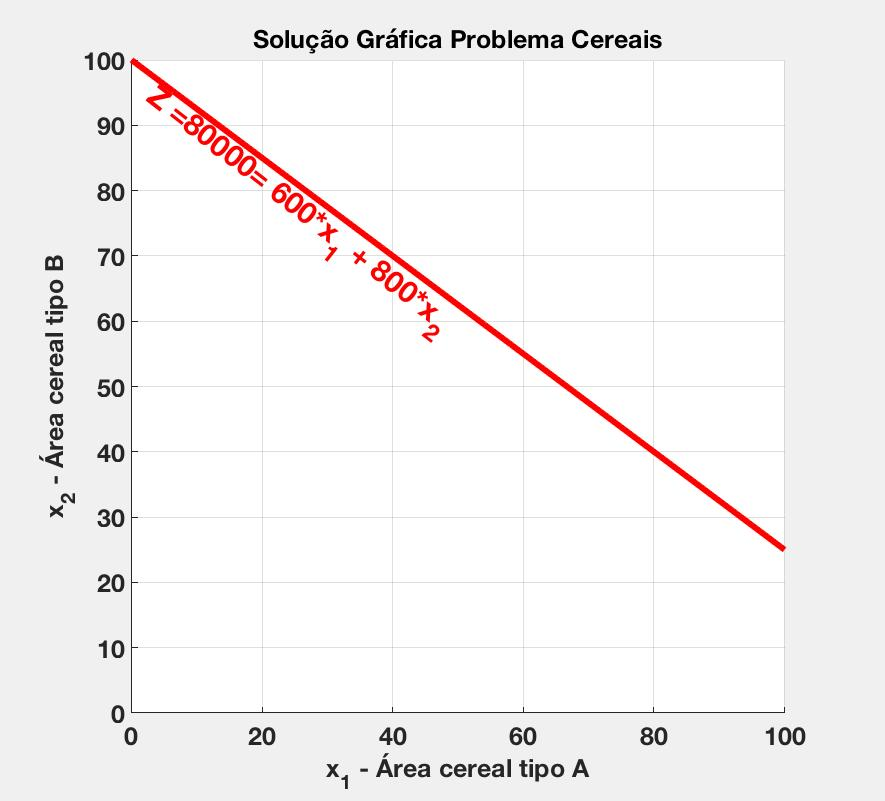
\includegraphics[width=6cm,height=6cm]{MatLab/anima_5.png} }
			\only<6> {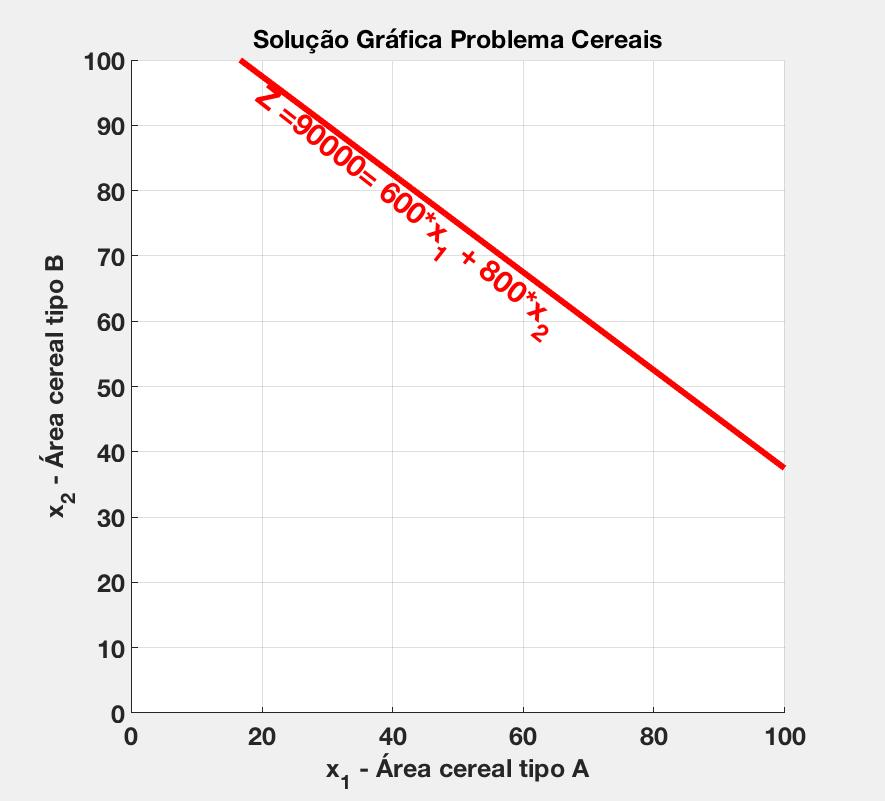
\includegraphics[width=6cm,height=6cm]{MatLab/anima_6.png} }
			\only<7> {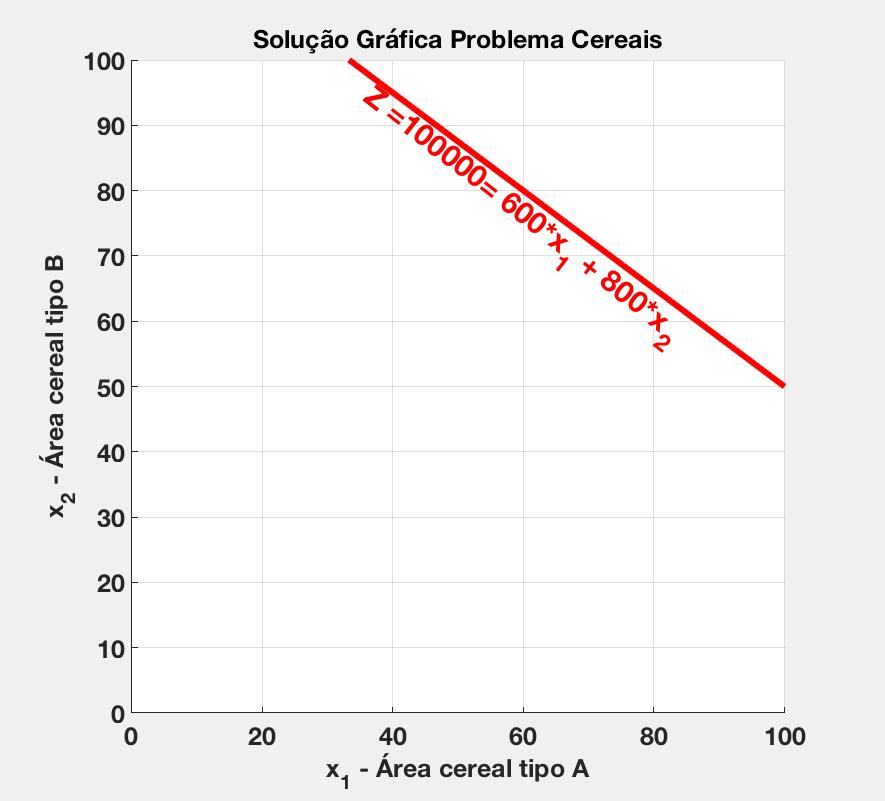
\includegraphics[width=6cm,height=6cm]{MatLab/anima_7.png} }
			\only<8> {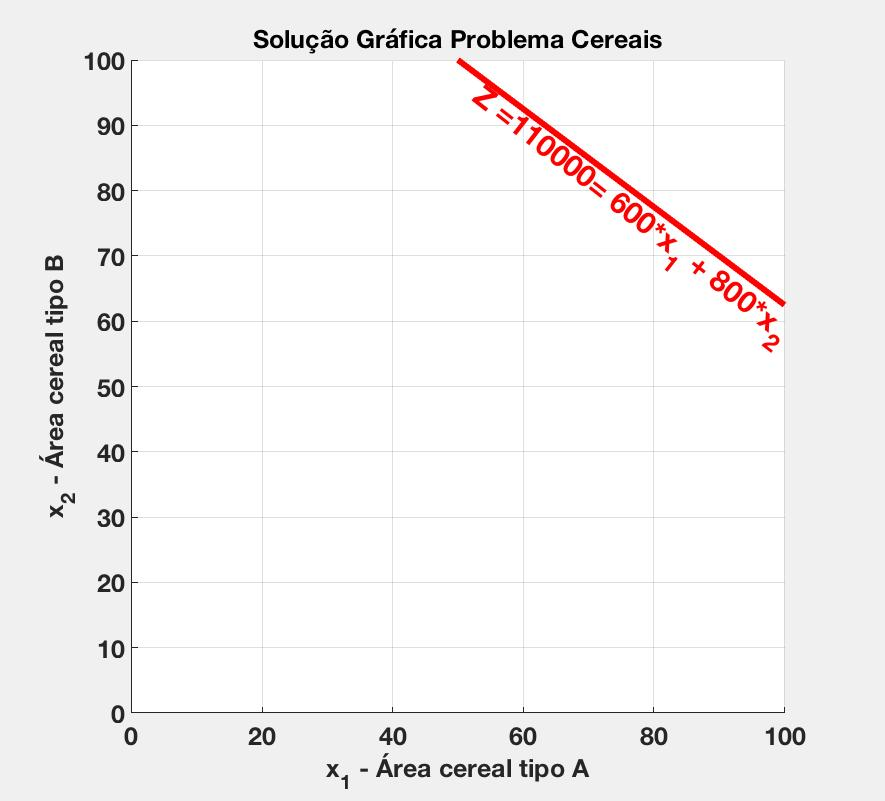
\includegraphics[width=6cm,height=6cm]{MatLab/anima_8.png} }
			\only<9-10> {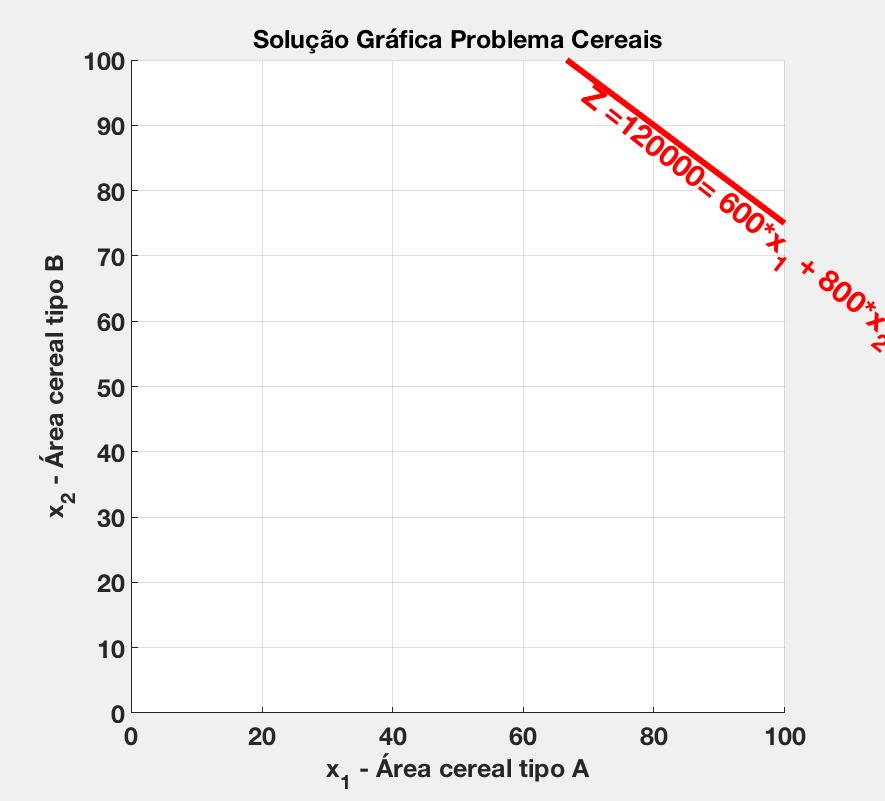
\includegraphics[width=6cm,height=6cm]{MatLab/anima_9.png} }
			\only<11-12> {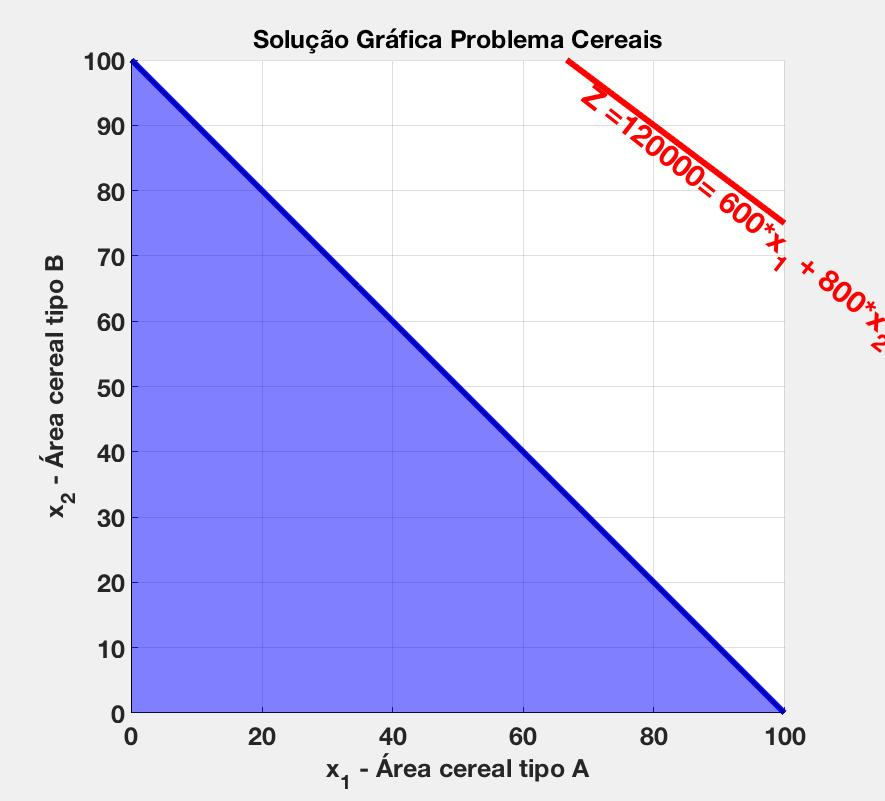
\includegraphics[width=6cm,height=6cm]{MatLab/anima_10.png} }
			\only<13> {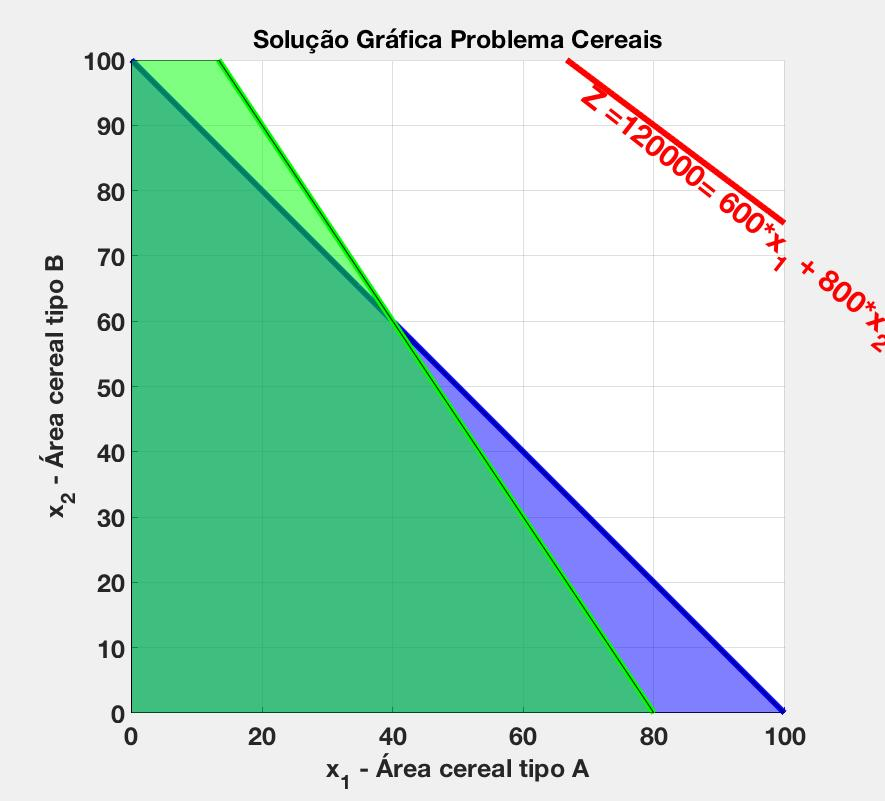
\includegraphics[width=6cm,height=6cm]{MatLab/anima_11.png} }
			\only<14-15> {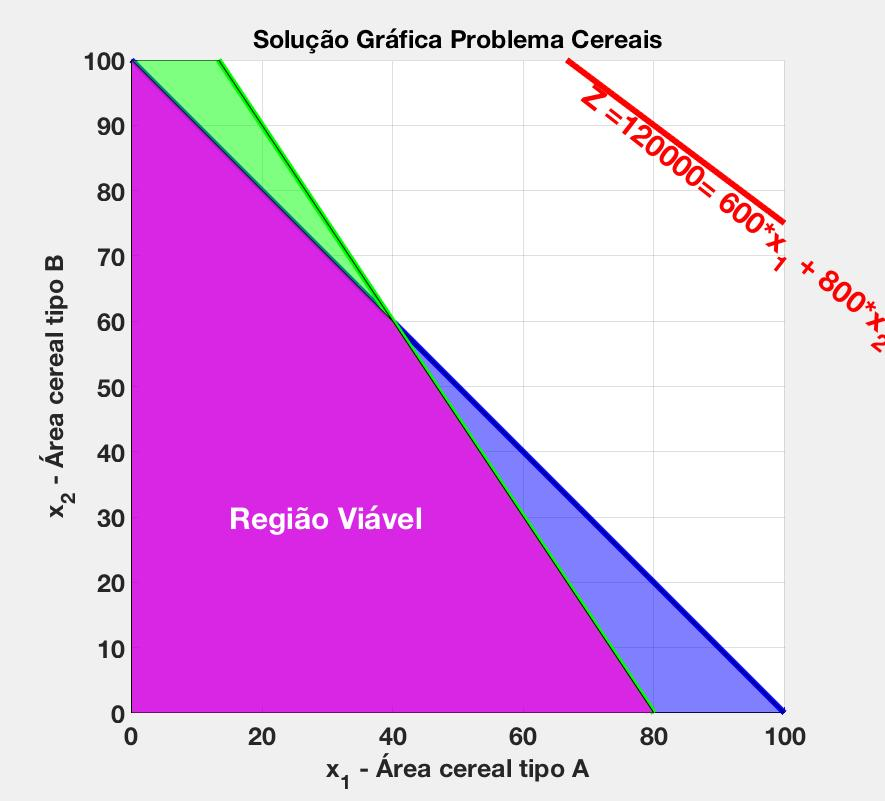
\includegraphics[width=6cm,height=6cm]{MatLab/anima_12.png} }
			\only<16> {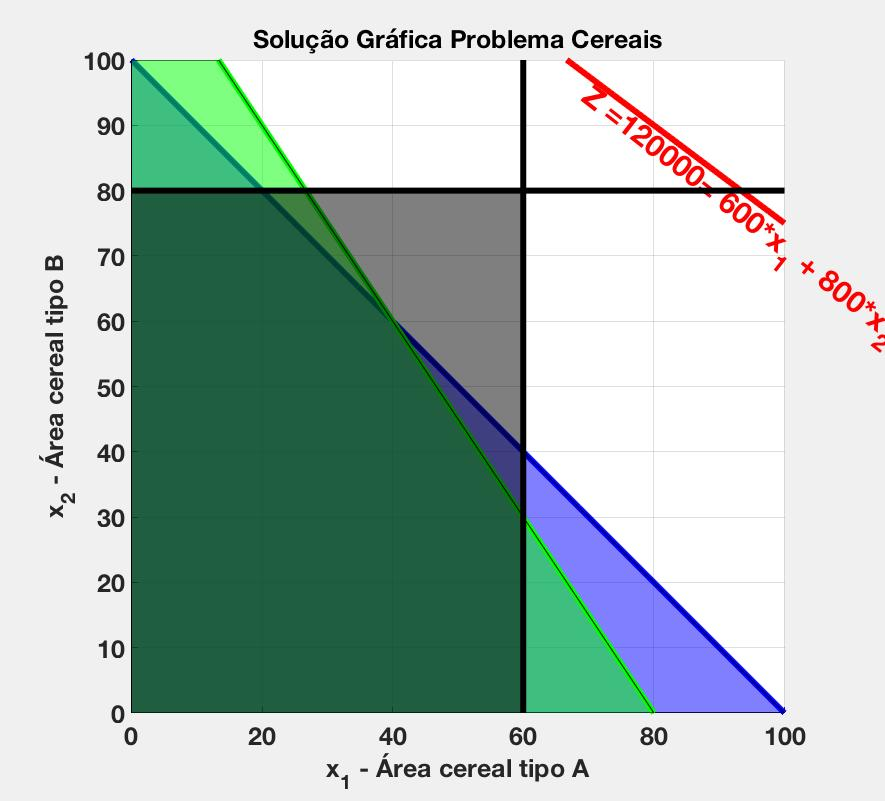
\includegraphics[width=6cm,height=6cm]{MatLab/anima_13.png} }
			\only<17> {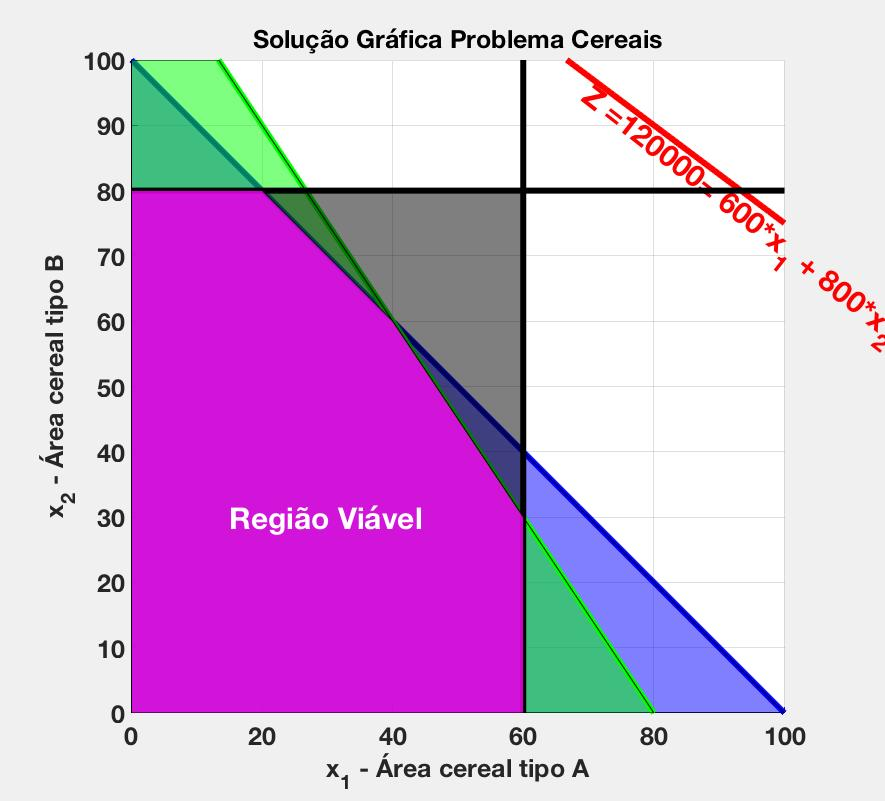
\includegraphics[width=6cm,height=6cm]{MatLab/anima_14.png} }
			\only<18> {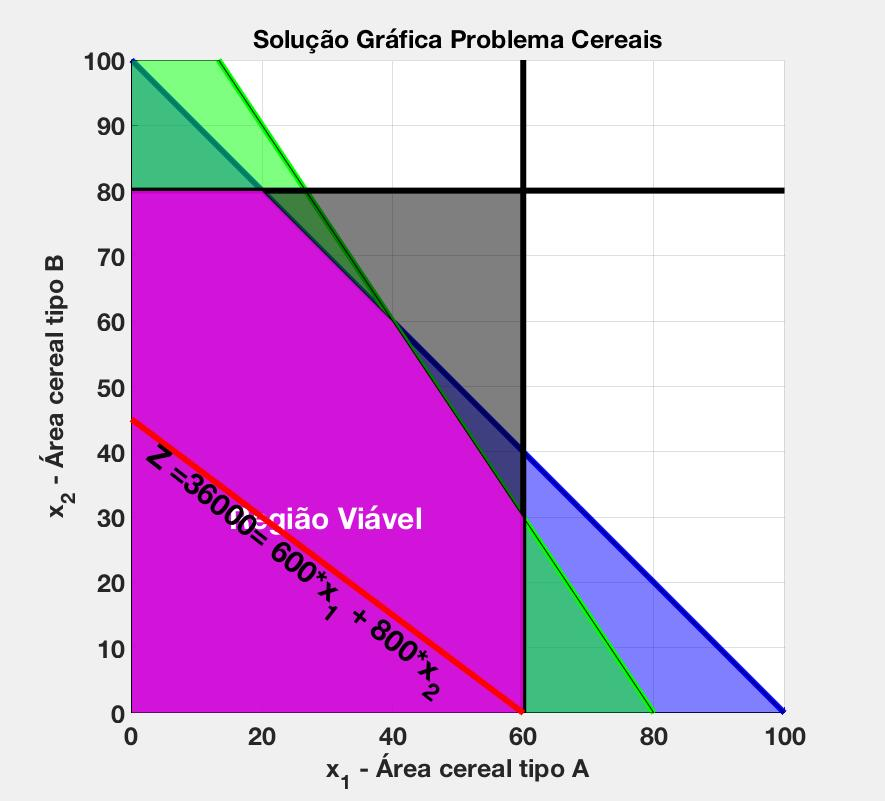
\includegraphics[width=6cm,height=6cm]{MatLab/anima_15.png} }
			\only<19> {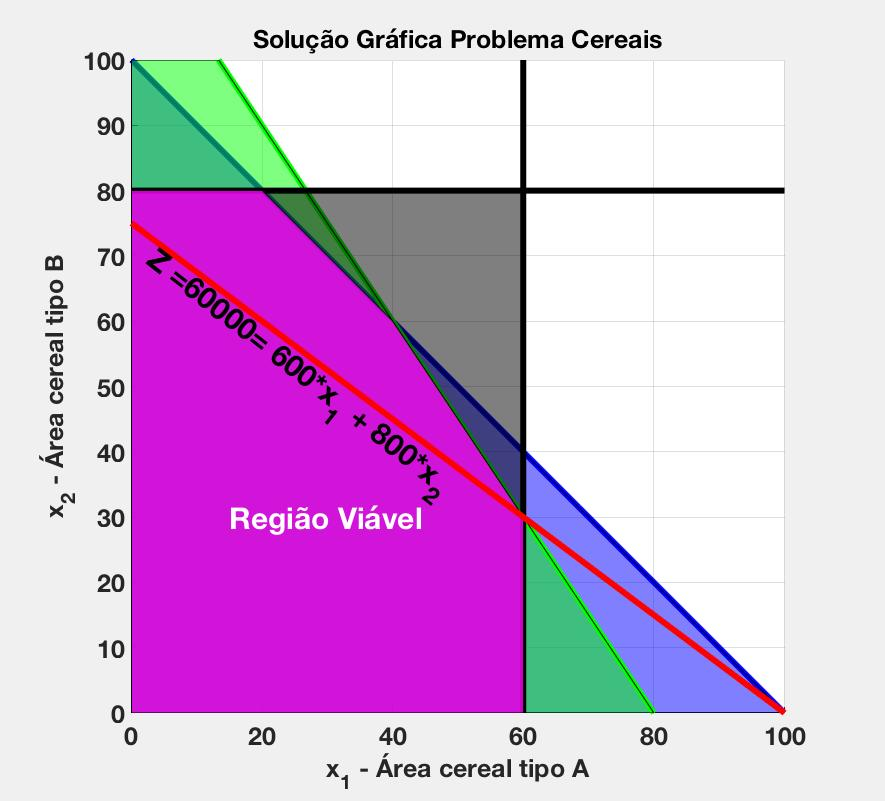
\includegraphics[width=6cm,height=6cm]{MatLab/anima_16.png} }
			\only<20> {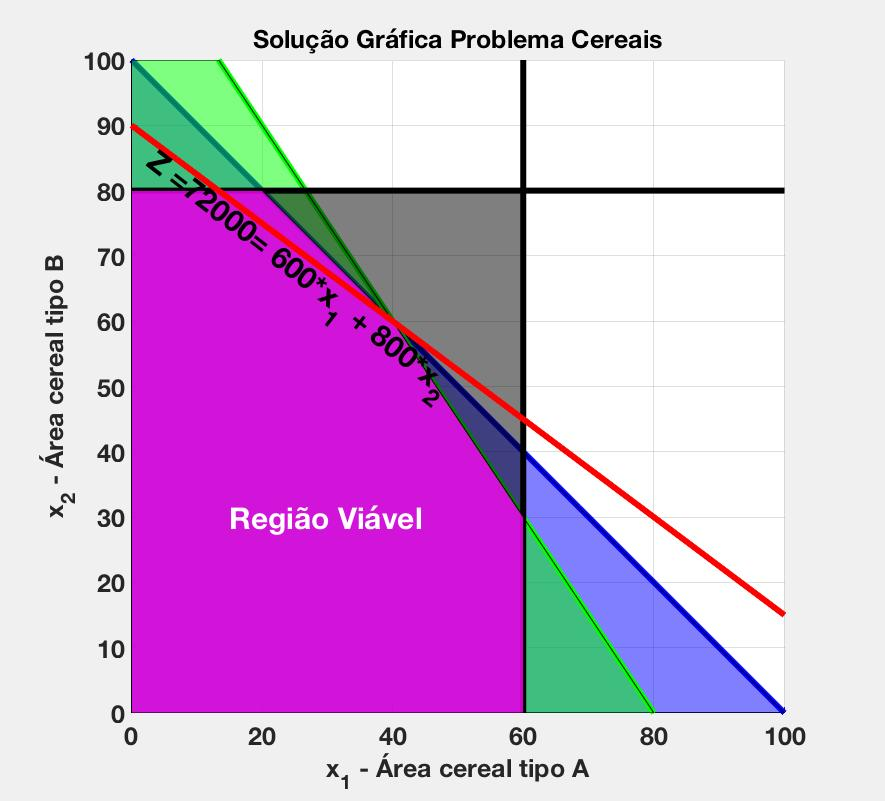
\includegraphics[width=6cm,height=6cm]{MatLab/anima_17.png} }
			\only<21-24> {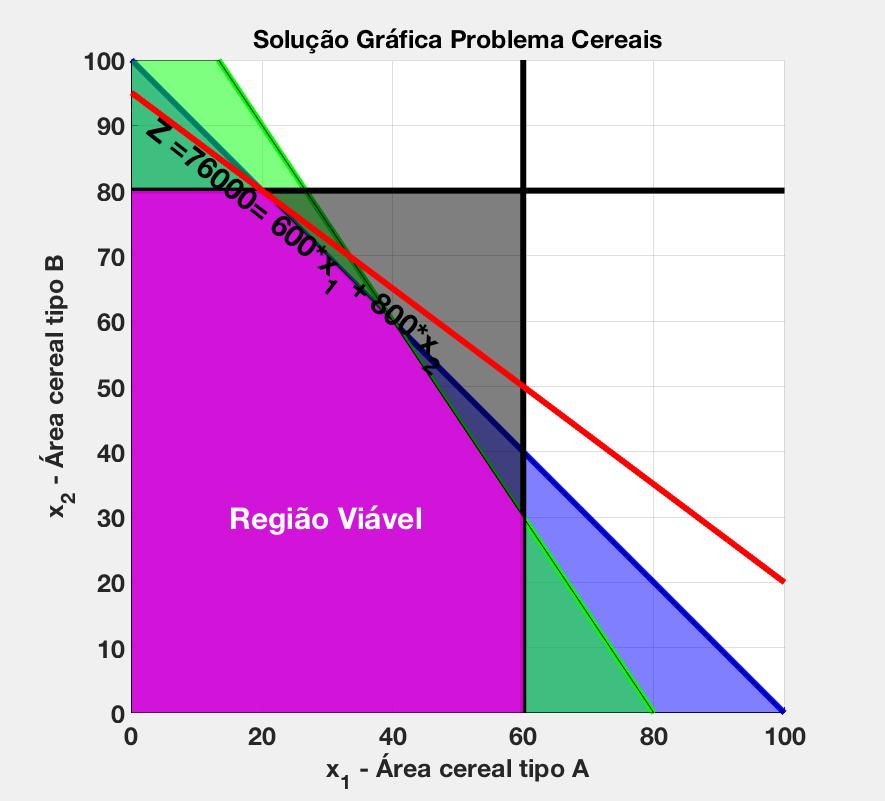
\includegraphics[width=6cm,height=6cm]{MatLab/anima_18.png} }
		\end{column}
	\end{columns}		
\end{frame}

\begin{frame}	
	\frametitle{Como achar a região viável?}
	\begin{columns}
		\begin{column}{0.5\textwidth}
			\begin{exampleblock}{Gradiente}
				\begin{itemize}
					\only<1-10> {\item[] $ \color{red}\max Z = 600x_1 + 800x_2$}
					\only<2-5> {\item[] \underline{Primeiro}: Determinar a direção do gradiente da \textbf{função objetivo}.}
					\only<3> {\item[] $ \nabla f(\mathbf{x}) = \begin{bmatrix}
																\frac{\partial f(\mathbf{x})}{\partial x_1} \\
																\frac{\partial f(\mathbf{x})}{\partial x_2} \\
																\vdots \\
																\frac{\partial f(\mathbf{x})}{\partial x_n} \\
															\end{bmatrix} $}
					\only<4-5> {\item[] O gradiente indica a direção do máximo crescimento da função.}
					\only<5> {\item[] $\nabla Z(x_1,x_2) = (600,800)$}
					\only<6-10> {\item[] \underline{Segundo}: {\color{red}Deslocar a função objetivo} na direção do gradiente da função, na busca da solução ótima do problema.}
					\only<10> {\item[] \color{red} \underline{Desafio:} Existem infinitos pares ($x_1$, $x_2$) viáveis!} 
				\end{itemize}
			\end{exampleblock}
			
		\end{column}
		\begin{column}{0.5\textwidth}
			\centering
			\only<1-3> {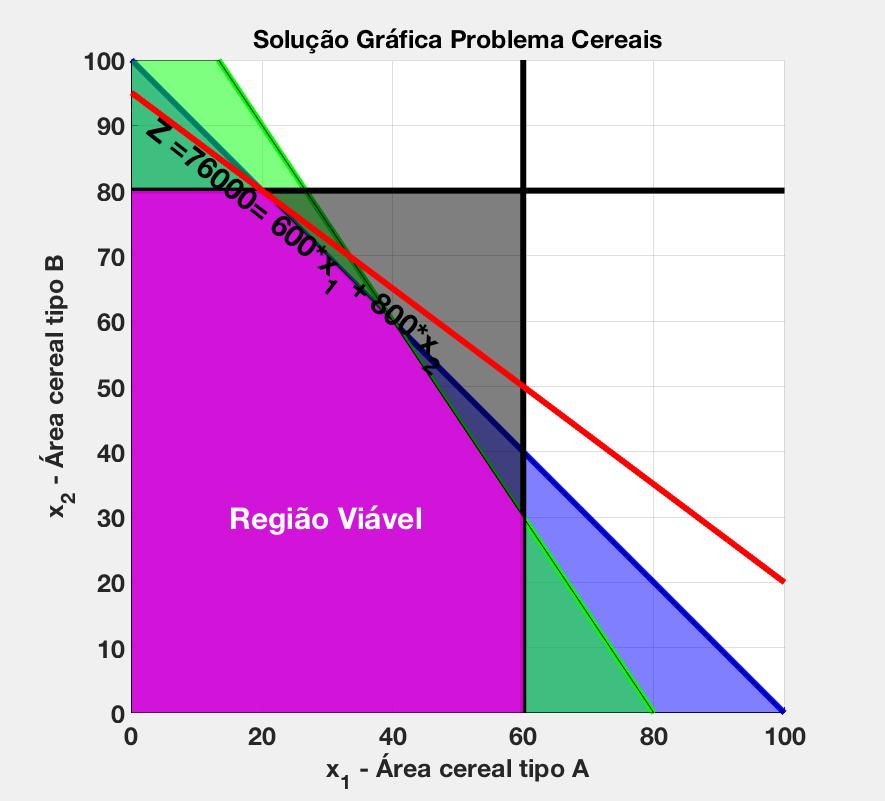
\includegraphics[width=6cm,height=6cm]{MatLab/anima_18.png} }
			\only<4-6> {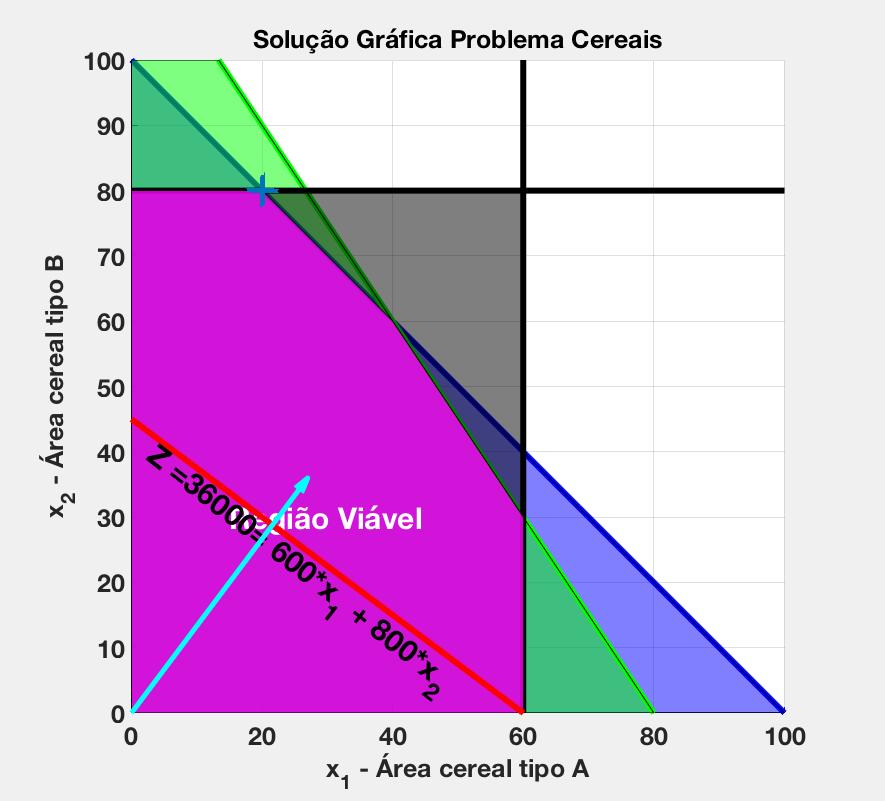
\includegraphics[width=6cm,height=6cm]{MatLab/anima_19.png} }
			\only<7> {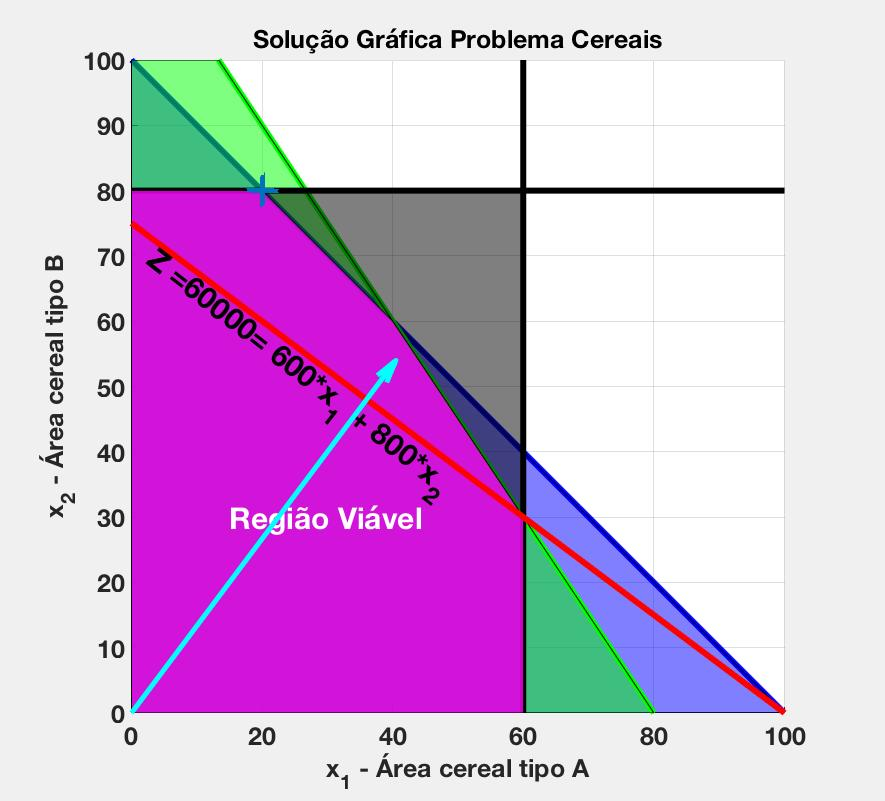
\includegraphics[width=6cm,height=6cm]{MatLab/anima_20.png} }
			\only<8> {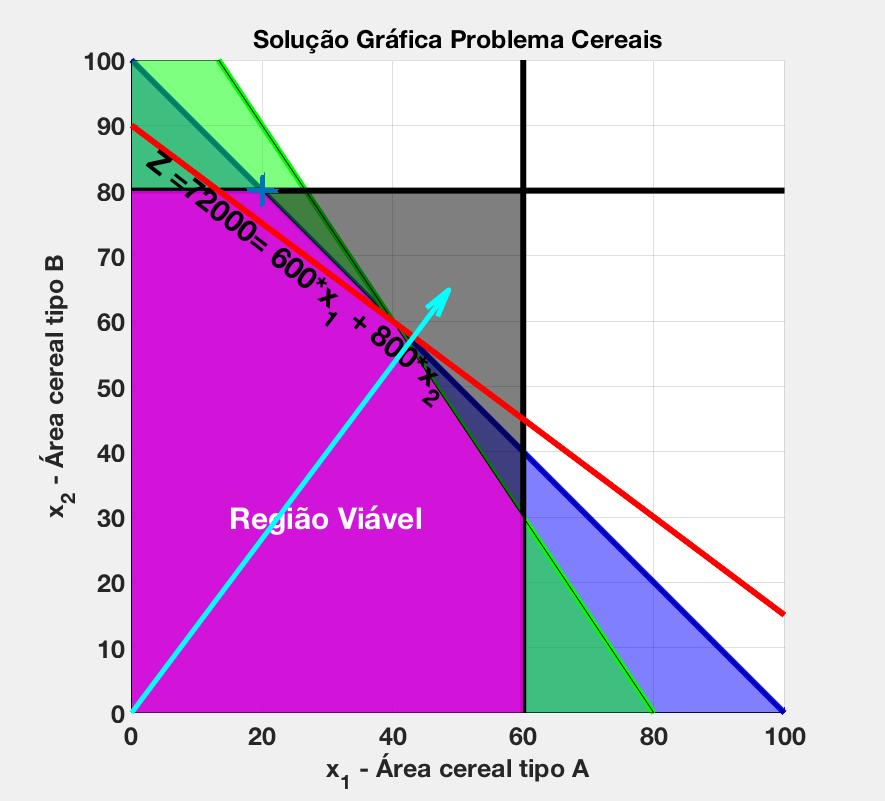
\includegraphics[width=6cm,height=6cm]{MatLab/anima_21.png} }
			\only<9-10> {\includegraphics[width=6cm,height=6cm]{MatLab/anima_22.png} }
		\end{column}
	\end{columns}
\end{frame}

\begin{frame}
	\frametitle{Análise Gráfica}
	\begin{block}{Teorema Fundamental da Programação Linear}
	A solução ótima de um problema de programação linear estará sempre em um dos vértices da região de solução do problema em análise. \only<3>{\footnote{\color{olive}Múltiplas Soluções ou Solução Ilimitada: Nestas situações a solução ótima pode não ser um vértice}}
	\end{block} 
	\only<2-3>{Os vértices correspondem às interseções de duas ou mais restrições.}
\end{frame}

\begin{frame}
	\frametitle{Solução Gráfica} 
	\centering
	\includegraphics[width=9cm,height=6cm]{ProblemaTrigoCereais.png}
\end{frame}

\begin{frame}
	\frametitle{Casos Especiais}
	\begin{itemize}
	\item Múltiplas Soluções
	\item Solução Infactível (Sem Solução)
	\item Solução Ilimitada
	\item Solução Degenerada
	\end{itemize}
\end{frame}

\begin{frame}
	\frametitle{Casos Especiais - Soluções Múltiplas}
	\centering
	\begin{columns}
		\begin{column}{0.3\textwidth}
			\begin{mdframed}[backgroundcolor=blue!20] 
				\scriptsize
				\begin{tabular}{l}
				$\max Z = 8x_1 + 4x_2$ \\
				s.a. \\
				$4x_1+2x_2 \le 16$ \\
				$x_1+x_2 \le 6$ \\
				$x_1, x_2 \ge 0 $ \\
				\end{tabular}
			\end{mdframed}
		\end{column}
		\begin{column}{0.7\textwidth}
			\includegraphics[width=8.5cm,height=7cm]{CasosEspeciais-Multiplas.png}
		\end{column}
	\end{columns}
	{\color{red}FOB Paralela a uma restrição ativa.}
\end{frame}

\begin{frame}
	\frametitle{Casos Especiais - Problema Sem Solução}
	\centering
	\begin{columns}
		\begin{column}{0.3\textwidth}
			\begin{mdframed}[backgroundcolor=blue!20] 
				\scriptsize
				\begin{tabular}{l}
				$\max Z = x_1 + x_2$ \\
				s.a. \\
				$5x_1+4x_2 \ge 40$ \\
				$2x_1+x_2 \le 6$ \\
				$x_1, x_2 \ge 0 $  \\
				\end{tabular}
			\end{mdframed}
		\end{column}
		\begin{column}{0.7\textwidth}
			\includegraphics[width=8.5cm,height=7cm]{CasosEspeciais-Infactivel.png}
		\end{column}
	\end{columns}
\end{frame}

\begin{frame}
	\frametitle{Casos Especiais - Prob. com Conj. Ilimitado de Soluções}
	\centering
	\begin{columns}
		\begin{column}{0.3\textwidth}
			\begin{mdframed}[backgroundcolor=blue!20] 		
				\scriptsize
				\begin{tabular}{l}
				$\max Z = 4x_1 + 3x_2$ \\
				s.a. \\
				$2x_1+5x_2 \ge 20$ \\
				$x_1 \le 8$ \\
				$x_1, x_2 \ge 0 $ \\ 
				\end{tabular}
			\end{mdframed}
		\end{column}
		\begin{column}{0.7\textwidth}
			\includegraphics[width=8.5cm,height=7cm]{CasosEspeciais-Ilimitado.png}
		\end{column}
	\end{columns}
\end{frame}

\begin{frame}
	\frametitle{Casos Especiais - Problema com Solução Degenerada}
	\centering
	\begin{columns}
		\begin{column}{0.3\textwidth}
			\begin{mdframed}[backgroundcolor=blue!20] 
				\scriptsize
				\begin{tabular}{l}
				$\max Z = x_1 + 5x_2$ \\
				s.a. \\
				$2x_1+4x_2 \ge 16$ \\
				$x_1+x_2 \le 6$ \\
				$x_1 \le 4$ \\
				$x_1, x_2 \ge 0 $ \\ 
				\end{tabular}
			\end{mdframed}
		\end{column}
		\begin{column}{0.7\textwidth}
			\includegraphics[width=8.5cm,height=7cm]{CasosEspeciais-Degenerada.png}
		\end{column}
	\end{columns}
	{\color{red}Existe no mínimo uma restrição redundante.}
\end{frame}


\section{Formulação Matricial}
\subsection{c, A, B, Aeq, Beq, lowerbound, upper bound}

\begin{frame}
	\frametitle{Formulação Matricial} 
	\begin{columns}
		\begin{column}{0.5\textwidth}
			\centering
			\begin{exampleblock}{Exemplo 1 - Problema do Agricultor/Área de Plantio}
				\scriptsize
				\begin{table}
					\begin{tabular}{r | l}
						{\color{red} $ \max Z = 600x_1+800x_2$ } & {\color{red} Objetivo } \\
						sujeito a & \\
						{\color{blue}$x_1+x_2 \le 100$} &  {\color{blue} Área} \\
						{\color{olive}$3x_1+2x_2 \le 240$} & {\color{olive}Mão de Obra} \\
						{$x_1 \le 60 $ } & {Produção \textbf{A} } \\
						{$x_2 \le 80 $ } &  {Produção  \textbf{B} } \\
						{$x_1, x_2 \ge 0$ } &  {Produção } \\
					\end{tabular}
				\end{table}
			\end{exampleblock}
			\includegraphics[width=1.5cm,height=2.3cm]{milho_aveia2.png}
		\end{column}
		\begin{column}{0.5\textwidth}
			\only<1>
			{
				\begin{equation*}
					 \max Z = \begin{bmatrix}
									800 & 600 \\ 
							 \end{bmatrix} 
					     	 \begin{bmatrix}
									 x_1 \\
									 x_2 \\
				    		 \end{bmatrix}
				\end{equation*}
				\begin{equation*}
					\begin{bmatrix}
							1 & 1 \\
							3 & 2 \\
							1 & 0  \\
							0 & 1 \\
					\end{bmatrix}
					\begin{bmatrix}
						x_1 \\
						x_2
					\end{bmatrix} \le
					\begin{bmatrix}
						100 \\
						240 \\
						60 \\
						80 \\
					\end{bmatrix}
				\end{equation*}
				\begin{equation*}
					x_1, x_2 \ge 0 
				\end{equation*}
			}
			\only<2>
			{
				\begin{equation*}
				\max Z = \overset{\mathbf{\color{red}c}}{\overbrace
								    {
									  \begin{bmatrix}
											800 & 600 \\ 
									  \end{bmatrix} 
									}
									}
						 \overset{\mathbf{\color{red}x}}{\overbrace
									{
									\begin{bmatrix}
										x_1 \\
										x_2 \\
									\end{bmatrix}
								  }
								  }
				\end{equation*}
				\begin{equation*}
					\underset{\mathbf{\color{red}A}}{\underbrace
								{
									\begin{bmatrix}
										1 & 1 \\
										3 & 2 \\
										1 & 0  \\
										0 & 1 \\
									\end{bmatrix}
								}}
					\underset{\mathbf{\color{red}x}}{\underbrace
								{
									\begin{bmatrix}
										x_1 \\
										x_2 \\
									\end{bmatrix} 
								}}
					\le
					\underset{\mathbf{\color{red}B}}{\underbrace
								{
									\begin{bmatrix}
										100 \\
										240 \\
										60 \\
										80 \\
									\end{bmatrix}
								}}
				\end{equation*}
				\begin{equation*}
				x_1, x_2 \ge 0 
				\end{equation*}
			}
			\only<3>
			{
				\centering
				\underline{\textbf{Notação Compacta}}
				\begin{equation*}
					\max Z = \mathbf{cx}
				\end{equation*} 
				\begin{equation*}
					\mathbf{Ax} \le \mathbf{B}
				\end{equation*}
				\begin{equation*}
					x_1, x_2 \ge 0 
				\end{equation*}
			}
		\end{column}
	\end{columns}		
\end{frame}

\begin{frame}
	\frametitle{Formulação Padrão Geral} 
	\begin{mdframed}[backgroundcolor=blue!20] 
		\only<1>
		{
			\begin{equation*}
				\max z = c_1x_1 + c_2x_2 + \cdots + c_nx_n 
			\end{equation*}
			{\color{red}Sujeito a (restrições de igualdade)} 
			\begin{equation*}
				\begin{matrix}
					a_{11}x_1 + a_{12}x_2 + \cdots + c_{1n}x_n = b_1 \\
					a_{21}x_1 + a_{22}x_2 + \cdots + c_{2n}x_n = b_2 \\
					\vdots \\
					a_{m1}x_1 + a_{m2}x_2 + \cdots + c_{mn}x_n = b_n \\
					x_1, x_2, \cdots, x_n \ge 0 \\
				\end{matrix}
			\end{equation*}
			$n$ variáveis de decisão e $m$ restrições de igualdade.
		}
		\only<2>
		{
			\begin{equation*}
				\max z = \sum_{j=1}^{n}c_jx_j
			\end{equation*}
			{\color{red}Sujeito a (restrições de igualdade)} 
			\begin{equation*}
				\begin{matrix}
					\sum_{j=1}^{n}a_{ij} = b_i & \forall i = 1, 2, \cdots, m \\
					x_j \ge 0 & \forall j = 1, 2, \cdots, n \\
				\end{matrix}
			\end{equation*}
			$n$ variáveis de decisão e $m$ restrições de igualdade.
		}
		\only<3>
		{
			\begin{equation*} 
				\max z = \begin{bmatrix}
							c_1 & c_2 & \cdots & c_n \\
						 \end{bmatrix}
						 \begin{bmatrix}
							 x_1 \\
							 x_2 \\
							 \vdots \\
							 x_n \\
						 \end{bmatrix}
			\end{equation*}
			{\color{red}Sujeito a (restrições de igualdade)} 
			\begin{equation*}
				\begin{bmatrix}
						a_{11} & a_{12} & \cdots & a_{1n} \\
						a_{21} & a_{22} & \cdots & a_{2n} \\
						\vdots & \vdots & \ddots & \vdots \\
						a_{m1} & a_{m2} & \cdots & a_{mn} \\
				\end{bmatrix}
				\begin{bmatrix}
						x_1 \\
						x_2 \\
						\vdots \\
						x_n \\
				\end{bmatrix} = 
				\begin{bmatrix}
						b_1 \\
						b_2 \\
						\vdots \\
						b_m \\
				\end{bmatrix} \text{ e }
				\begin{bmatrix}
						x_1 \\
						x_2 \\
						\vdots \\
						x_n \\
				\end{bmatrix} \ge
				\begin{bmatrix}
						0 \\
						0 \\
						\vdots \\
						0 \\
				\end{bmatrix} 				
			\end{equation*}			
			$n$ variáveis de decisão e $m$ restrições de igualdade.
		}
		\only<4>
		{
			\begin{equation*} 
				\max z = \begin{bmatrix}
							c_1 & c_2 & \cdots & c_n \\
						 \end{bmatrix}_{\text{\color{red}1 x n}}
						 \begin{bmatrix}
							 x_1 \\
							 x_2 \\
							 \vdots \\
							 x_n \\
						 \end{bmatrix}_{\text{\color{red}n x 1}} 
			\end{equation*}
			{\color{red}Sujeito a (restrições de igualdade)} 
			\begin{equation*}
				\begin{bmatrix}
						a_{11} & a_{12} & \cdots & a_{1n} \\
						a_{21} & a_{22} & \cdots & a_{2n} \\
						\vdots & \vdots & \ddots & \vdots \\
						a_{m1} & a_{m2} & \cdots & a_{mn} \\
				\end{bmatrix}_{\text{\color{red}m x n}}
				\begin{bmatrix}
						x_1 \\
						x_2 \\
						\vdots \\
						x_n \\
				\end{bmatrix}_{\text{\color{red} n x 1}} = 
				\begin{bmatrix}
						b_1 \\
						b_2 \\
						\vdots \\
						b_m \\
				\end{bmatrix}_{\text{\color{red} m x 1}}  				
			\end{equation*}			
			$n$ variáveis de decisão e $m$ restrições de igualdade.
		}
		\only<5>
		{
			\begin{equation*} 
				\max z = \mathbf{c}^T \mathbf{x}
			\end{equation*}
			{\color{red}Sujeito a (restrições de igualdade)} 
			\begin{equation*}
				\begin{matrix}
					\mathbf{A_{eq}x} = \mathbf{B_{eq}}  \\
					\mathbf{x} \ge \mathbf{0}
				\end{matrix}
			\end{equation*}	
			$n$ variáveis de decisão e $m$ restrições de igualdade.		
		}		
	\end{mdframed}
	\only<5>
	{
	\vspace{0.3cm}
	\begin{equation*}
		\begin{matrix}
			\mathbf{c} = 	\begin{bmatrix}
									c_1 \\ c_2 \\ \vdots \\ c_n \\
							\end{bmatrix} &

			\mathbf{x} = 	\begin{bmatrix}
									x_1 \\ x_2 \\ \vdots \\ x_n \\
							\end{bmatrix} &

			\mathbf{B_{eq}} = 	\begin{bmatrix}
									b_1 \\ b_2 \\ \vdots \\ b_m \\
							\end{bmatrix} &

			\mathbf{A_{eq}} = 	\begin{bmatrix}
									a_{11} & a_{12} & \cdots & a_{1n} \\
									a_{21} & a_{22} & \cdots & a_{2n} \\
									\vdots & \vdots & \ddots & \vdots \\
									a_{m1} & a_{m2} & \cdots & a_{mn} \\
								\end{bmatrix} \\

		\end{matrix}
	\end{equation*}
	}
\end{frame}

\begin{frame}
	\frametitle{Relação entre Maximização e Minimização}
	\only<1>
	{
		\centering
		\includegraphics[width=5cm,height=4cm]{up-down.jpg}
	}	
	\only<2>
	{
		\centering
		\includegraphics[width=5cm,height=4cm]{up-down.jpg}
		\begin{itemize}
		\item Qualquer que seja o formato do PPL, sempre é possível transforma-lo no formato padrão apresentado.
		\item Como é a relação entre minimização e maximização?
		\end{itemize}
	}	
	\only<3>
	{
		\centering
		\includegraphics[width=2.5cm,height=2cm]{up-down.jpg}
		\begin{mdframed}[backgroundcolor=blue!20] 
			\begin{equation*}
				\max z = \sum_{j=1}^{n}c_jx_j \Leftrightarrow \min (-z) = \sum_{j=1}^{n}(-c_j)x_j
			\end{equation*}
			\begin{equation*}
				\min z = \sum_{j=1}^{n}c_jx_j \Leftrightarrow \max (-z) = \sum_{j=1}^{n}(-c_j)x_j
			\end{equation*}
		\end{mdframed}
	}
\end{frame}

\begin{frame}
	\frametitle{Relação Entre Inequações e Equações}
	
	\only<1->
	{
	\underline{Restrições de Menor ou Igual}
	\begin{mdframed}[backgroundcolor=blue!20]
		\begin{equation*}
			\sum_{j-1}^{n}a_{ij} \le b_i \Leftrightarrow
			\left\{ \begin{matrix}
						\sum_{j=1}^{n}a_{ij}x_j + S_i = b_i \\
						0 \le S_i \ge \infty
					\end{matrix}  
			\right.
		\end{equation*}
	\end{mdframed}	
	}
	
	\only<2>
	{
	\vspace{0.5cm}
	\underline{Restrições de Maior ou Igual}
	\begin{mdframed}[backgroundcolor=red!20]
		\begin{equation*}
			\sum_{j-1}^{n}a_{ij} \ge b_i \Leftrightarrow
			\left\{ \begin{matrix}
						\sum_{j=1}^{n}a_{ij}x_j - S_i = b_i \\
						0 \le S_i \ge \infty
					\end{matrix}  
			\right.
		\end{equation*}
	\end{mdframed}
	}
\end{frame}

\begin{frame}
	\frametitle{Tratamento de Limites das Variáveis}
	\only<1->
	{
	\underline{Limite Inferior ou \textit{Lower  Bound}}
	\begin{mdframed}[backgroundcolor=blue!20]
		\begin{equation*}
			x_j \ge LB \Leftrightarrow
			\left\{ \begin{matrix}
						x_j - LB = {x}'_j \Rightarrow x_j = {x}'_j + LB \\
						{x}'_j \ge 0
					\end{matrix}  
			\right.
		\end{equation*}
	\end{mdframed}	
	}
	
	\only<2->
	{
	\vspace{0.5cm}
	\underline{Limite Superior ou \textit{Upper  Bound}}
	\begin{mdframed}[backgroundcolor=red!20]
		\begin{equation*}
			x_j \le UB \Leftrightarrow
			\left\{ \begin{matrix}
						UB - x_j = {x}'_j \Rightarrow x_j = UB - {x}'_j  \\
						{x}'_j \ge 0
					\end{matrix}  
			\right.
		\end{equation*}
	\end{mdframed}
	}

	\only<3->
	{
	\vspace{0.5cm}
	\begin{mdframed}[backgroundcolor=green!20]
		\begin{equation*}
			- \infty \le x_j \le \infty \Leftrightarrow
			\left\{ \begin{matrix}
						x_j = {x}'_j - {x}''_j \\
						{x}'_j \ge 0 \text{ e } {x}''_j \ge 0  \\
					\end{matrix}  
			\right.
		\end{equation*}
	\end{mdframed}
	}
\end{frame}

\begin{frame}
	\frametitle{Observações}
	\begin{itemize}
	\item As restrições do problema expressam limites que devem ser respeitados
	\item {O algoritmo de resolução encontra a solução ótima no espaço de soluções compatíveis com o problema de PL, a saber:}
		\begin{itemize}
		\item Os pontos pertencentes a região factível correspondem aos valores das variáveis que atendem ao conjunto de restrições;
		\item Cada restrição poderá ser de igualdade ou desigualdade
		\item As restrições de não-negatividade das variáveis constituem condição necessária à aplicação do algoritmo de resolução do problema de PL;
		\item Embora isso normalmente ocorra em decorrência da natureza da variável dentro do modelo, pode haver situações em que as variáveis são irrestritas, isto é, podem assumir qualquer valor real (nestes casos, realizar substituição de variáveis).
		\end{itemize}
	\end{itemize}
\end{frame}

\begin{frame}
	\frametitle{Softwares de Otimização }
	\centering
	\begin{table}
		\begin{tabular}{c c c c}
		\includegraphics[width=2cm,height=2cm]{solver_matlab.png} & 
		\includegraphics[width=2cm,height=2cm]{solver_coin.png} &
		\includegraphics[width=2cm,height=2cm]{solver_cplex.jpg} &
		\includegraphics[width=2cm,height=2cm]{solver_ampl.jpg} \\
		\includegraphics[width=2cm,height=2cm]{solver_excel.png} & 
		\includegraphics[width=2cm,height=2cm]{solver_gams.png} &
		\includegraphics[width=2cm,height=2cm]{solver_R.png} &		
		\includegraphics[width=2cm,height=2cm]{solver_gurobi.png} \\
		\includegraphics[width=2cm,height=2cm]{solver_lingo.png} & 
		\includegraphics[width=2cm,height=2cm]{solver_python.jpg} &
		\includegraphics[width=2cm,height=2cm]{solver_julia.png} &
		\includegraphics[width=4cm,height=2cm]{solver_xpress.png} \\		
		\end{tabular}
	\end{table}
\end{frame}
	
\begin{frame}
	\frametitle{Toolbox de Programação Linear do Matlab}
	\begin{table}
		\begin{tabular}{c}
			\only<1-4>
			{
				\includegraphics[width=2cm,height=2cm]{solver_matlab.png} \\
			}
			\only<1>
			{
				\includegraphics[width=7cm,height=5cm]{linprogA.png} \\
			}
			\only<2>
			{
				\includegraphics[width=7cm,height=5cm]{linprogA1.png}\\
			}
			\only<3>
			{
				\includegraphics[width=7cm,height=5cm]{linprogB.png}\\
			}
			\only<4>
			{
				\begin{tabular}{| l |}
					\hline
					\cellcolor{yellow} Parâmetros de Entrada \\
					\hline
					\cellcolor{green!20} f: Vetor de Custos \\
					\cellcolor{gray!20} A: Matriz dos coeficientes das restrições de desiguadade \\
					\cellcolor{green!20} b: Termos constantes das restrições de desigualdade \\
					\cellcolor{gray!20} Aeq: Matriz dos coeficientes das restrições de igualdade \\
					\cellcolor{green!20} Beq: Termos constantes das restrições de igualdade \\
					\cellcolor{gray!20} lb: Vetor com os limites inferiores das variáveis \\
					\cellcolor{green!20} ub: Vetor com os limites superiores das variáveis \\
					\cellcolor{gray!20} options: Configuração do comportamento do solver \\
					\hline
				\end{tabular}
			}
			\only<5>
			{
				\begin{tabular}{| l |}
					\hline
					\cellcolor{yellow} Parâmetros de Saída \\
					\hline
					\cellcolor{green!20} x: Vetor os valores ótimos das variáveis \\
					\cellcolor{gray!20} fval: Valor da Função Objetivo \\
					\cellcolor{green!20} exitflag: Código detalhando processo de convergência: \\
						\hspace{0.4cm}\scriptsize\cellcolor{green!20} (1) Função convergiu para a solução x \\
						\hspace{0.4cm}\scriptsize\cellcolor{green!20} (0) Número de iterações excedido. options.MaxIterations \\
						\hspace{0.4cm}\scriptsize\cellcolor{green!20} (-2) Não foi encontrato um x viável \\
						\hspace{0.4cm}\scriptsize\cellcolor{green!20} (-3) Problema é ilimitado \\
						\hspace{0.4cm}\scriptsize\cellcolor{green!20} (-4) Encontrada divisão por zero durante processo \\
						\hspace{0.4cm}\scriptsize\cellcolor{green!20} (-5) Tanto o primal quando dual são inviáveis \\
						\hspace{0.4cm}\scriptsize\cellcolor{green!20} (-7) Direção de busca tornou-se pequena demais. \\ 
					\cellcolor{gray!20} output: Informações sobre do processo de otimização \\
					\cellcolor{green!20} lambda: Multiplicadores de lagrange da solução \\
					\hline
				\end{tabular}
			}

		\end{tabular}
	\end{table}
\end{frame}

\begin{frame}
	\frametitle{Problema do Milho e da Aveia}
	\begin{columns}
		\begin{column}{0.7\textwidth}
			\centering
			\begin{exampleblock}{Exemplo 1 - Modelo Matemático Completo}
				\scriptsize
				\begin{table}
					\begin{tabular}{r c l}
						$ \max Z = 600x_1+800x_2$ & \includegraphics[width=0.8cm,height=0.2cm]{seta2.png} & Função Objetivo \\
						sujeito a & & \\
						$x_1+x_2 \le 100$ & \includegraphics[width=0.8cm,height=0.2cm]{seta2.png}& Área Cultivo \\
						$3x_1+2x_2 \le 240$ & \includegraphics[width=0.8cm,height=0.2cm]{seta2.png}& Mão de Obra \\
						$x_1 \le 60 $ & \includegraphics[width=0.8cm,height=0.2cm]{seta2.png}& Produção Cereal \textbf{A} \\
						$x_2 \le 80 $ &\includegraphics[width=0.8cm,height=0.2cm]{seta2.png} & Produção Cereal \textbf{B} \\
						$x_1, x_2 \ge 0$ & \includegraphics[width=0.8cm,height=0.2cm]{seta2.png}& Produção \\
					\end{tabular}
				\end{table}
			\end{exampleblock}
		\end{column}
		\begin{column}{0.3\textwidth}
			\centering
			\includegraphics[width=2cm,height=3cm]{milho_aveia2.png}
		\end{column}
	\end{columns}
	\begin{mdframed}[backgroundcolor=blue!20]
		\Large
		Confirmar o resultado da Análise Gráfica com o Matlab !
	\end{mdframed}	
\end{frame}

\begin{frame}[fragile] 
	\frametitle{Problema do Milho e da Aveia}
	\centering
	\begin{block}{Programa em Matlab}
		\begin{lstlisting}
clear all; close all; clc;
f = [-600 -800]; A = [1 1; 3 2]; b = [100; 240];
Aeq=[]; beq=[]; LB=[0 0]; UB=[60 80];
[x, fval, exitflag] = linprog(f,A,b,Aeq,beq,LB,UB)		
		\end{lstlisting}	
	\end{block}	

	\begin{figure}
		\includegraphics[width=3.5cm,height=4.5cm]{MatLabTriboAveia.png}
	\end{figure}

\end{frame}

\begin{frame}
	\frametitle{Análise Gráfica x Matlab}
	\centering
	\includegraphics[width=10cm,height=7cm]{graficamatlab.png}
\end{frame}


\section{Mais Exemplos}

\subsection{Aviário}

\begin{frame}
	\frametitle{Exemplo Aviário}
	\begin{block}{O problema}
		\scriptsize
		O dono de um aviário precisa fabricar uma ração especial para as suas aves, de forma a atender diversas exigências alimentares. A produção desejada de ração é de 90kg, e a mistura deve ser formada por dois ingredientes básicos: milho e farelo de arroz, que custam \$0,90 e \$0,30 por kg respectivamente. Além disso, sabe-se que a ração precisa ter pelo menos 7\% de proteína e 3\% de fibra na sua composição, de forma a atender as necessidades das aves. A partir da tabela abaixo, com a composição percentual de fibra e proteína do milho e do farelo de arroz, pede-se formular um problema de programação linear para atender às necessidades diárias a um custo mínimo. 
	\end{block}
	\begin{columns}
		\begin{column}{0.7\textwidth}
			\begin{table}
				\scriptsize
				\caption{Composição de Cada Ingrediente}
				\begin{tabular}{| c | c | c |}
					\hline
					\textbf{Ingredientes} & \textbf{Proteína} & \textbf{Fibra} \\
					\hline
					Milho				  & 9 \%              & 2 \% \\
					Farelo de Arroz		  & 5 \%			  & 6 \% \\
					\hline
				\end{tabular}
			\end{table}
		\end{column}
		\begin{column}{0.3\textwidth}
				\centering
				\includegraphics[width=2cm,height=3cm]{aviario.jpg}
		\end{column}
	\end{columns}
\end{frame}

\begin{frame}
	\frametitle{Exemplo Aviário}
	\begin{columns}
		\begin{column}{0.8\textwidth}
			\centering
			\begin{exampleblock}{Exemplo 1 - Modelo Matemático Completo}
				\centering
				\scriptsize
				\begin{table}
					\only<1>
					{
					\begin{tabular}{r c l}
						$ \min Z = 0.9x_M+0.3x_F$ & \includegraphics[width=0.8cm,height=0.2cm]{seta2.png} & Minimizar Custo \\
						sujeito a & & \\
						$1x_M+1x_F = 90$ & \includegraphics[width=0.8cm,height=0.2cm]{seta2.png}& Produção \\
						$0.09x_M+0.05x_F \ge 0.07(x_M+x_F)$ & \includegraphics[width=0.8cm,height=0.2cm]{seta2.png}& Proteína \\
						$0.02x_M+0.06x_F \ge 0.03(x_M+x_F)$ & \includegraphics[width=0.8cm,height=0.2cm]{seta2.png}& Fibra \\
						$x_M, x_F \ge 0$ & \includegraphics[width=0.8cm,height=0.2cm]{seta2.png}& Canalização \\
					\end{tabular}
					}
					\only<2>
					{
					\begin{tabular}{r c l}
						$ \min Z = 0.9x_M+0.3x_F$ & \includegraphics[width=0.8cm,height=0.2cm]{seta2.png} & Minimizar Custo \\
						sujeito a & & \\
						$1x_M+1x_F = 90$ & \includegraphics[width=0.8cm,height=0.2cm]{seta2.png}& Produção \\
						$0.02x_M-0.02x_F \ge 0$ & \includegraphics[width=0.8cm,height=0.2cm]{seta2.png}& Proteína \\
						$-0.01x_M+0.03x_F \ge 0$ & \includegraphics[width=0.8cm,height=0.2cm]{seta2.png}& Fibra \\
						$x_M, x_F \ge 0$ & \includegraphics[width=0.8cm,height=0.2cm]{seta2.png}& Canalização \\
					\end{tabular}
					}					
				\end{table}
				\only<3>
				{	
					Função Objetivo \\~\\
					\includegraphics[width=6cm,height=6cm]{MatLab/aviario_1.png}
				}
				\only<4>
				{	
					Função Objetivo \\~\\
					\includegraphics[width=6cm,height=6cm]{MatLab/aviario_2.png}
				}
				\only<5>
				{	
					Função Objetivo \\~\\
					\includegraphics[width=6cm,height=6cm]{MatLab/aviario_3.png}
				}
				\only<6>
				{	
					Função Objetivo \\~\\
					\includegraphics[width=6cm,height=6cm]{MatLab/aviario_4.png}
				}
				\only<7>
				{	
					Função Objetivo \\~\\
					\includegraphics[width=6cm,height=6cm]{MatLab/aviario_5.png}
				}
				\only<8>
				{	
					Função Objetivo \\~\\
					\includegraphics[width=6cm,height=6cm]{MatLab/aviario_6.png}
				}
				\only<9>
				{	
					Função Objetivo \\~\\
					\includegraphics[width=6cm,height=6cm]{MatLab/aviario_7.png}
				}
				\only<10>
				{	
					Função Objetivo \\~\\
					\includegraphics[width=6cm,height=6cm]{MatLab/aviario_8.png}
				}
				\only<11>
				{	
					Função Objetivo \\~\\
					\includegraphics[width=6cm,height=6cm]{MatLab/aviario_9.png}
				}
				\only<12>
				{	
					Restrição de Igualdade: $1x_M+1x_F = 90$ \\~\\
					\includegraphics[width=6cm,height=6cm]{MatLab/aviario_10.png}
				}
				\only<13>
				{	
					Restrição Proteína: $0.02x_M-0.02x_F \ge 0$  \\~\\
					\includegraphics[width=6cm,height=6cm]{MatLab/aviario_11.png}
				}
				\only<14>
				{	
					Restrição Fibra: $-0.01x_M+0.03x_F \ge 0$ \\~\\
					\includegraphics[width=6cm,height=6cm]{MatLab/aviario_12.png}
				}
				\only<15>
				{	
					Minimizando Função Objetivo \\~\\
					\includegraphics[width=6cm,height=6cm]{MatLab/aviario_13.png}
				}
				\only<16>
				{	
					Minimizando Função Objetivo \\~\\
					\includegraphics[width=6cm,height=6cm]{MatLab/aviario_14.png}
				}
				\only<17>
				{	
					Minimizando Função Objetivo \\~\\
					\includegraphics[width=6cm,height=6cm]{MatLab/aviario_15.png}
				}
				\only<18>
				{	
					Minimizando Função Objetivo \\~\\
					\includegraphics[width=6cm,height=6cm]{MatLab/aviario_16.png}
				}
				\only<19>
				{	
					Ponto Ótimo Global \\~\\
					\includegraphics[width=6cm,height=6cm]{MatLab/aviario_17.png}
				}
			\end{exampleblock}
		\end{column}
		\begin{column}{0.2\textwidth}
			\centering
			\includegraphics[width=2cm,height=3cm]{aviario.jpg}
		\end{column}
	\end{columns}
	\only<1-2>
	{
	\begin{mdframed}[backgroundcolor=blue!20]
		\Large
		Confirmar o resultado da Análise Gráfica com o Matlab !
	\end{mdframed}
	}	
\end{frame}

\begin{frame}[fragile] 
	\frametitle{Exemplo Aviário}
	\centering
	\begin{block}{Programa em Matlab}
		\begin{lstlisting}
clear all; close all; clc;
f = [0.9 0.3]; A = [-0.02 0.02;0.01 -0.03]; 
B = [ 0; 0]; Aeq = [ 1 1 ]; Beq = 90;
[x, fval] = linprog(f,A,B,Aeq,Beq)	
		\end{lstlisting}	
	\end{block}	

	\begin{figure}
		\includegraphics[width=3.5cm,height=4.5cm]{MatLabAviario.png}
	\end{figure}

\end{frame}

\subsection{Produção}
\begin{frame}
	\frametitle{Empresa e seus Produtos}
	\begin{block}{O problema}
		\scriptsize
		Seja uma empresa que produz produtos A, B, C e D. A fabricação de cada unidade desses produtos exige mão de obra, matéria-prima e processamento mecânico, gerando um dado lucro de acordo com a Tabela abaixo.
		\\~\\
		O suprimento semanal de matéria prima é restrito a 20.000Kg. A disponibilidade semanal de mão de obra é de 15.000 horas, e a quantidade de horas-máquina é de 40.000 hm. Pede-se determinar o plano de produção semanal de forma a maximizar o lucro. 
	\end{block}
	\begin{columns}
		\begin{column}{0.7\textwidth}
			\begin{table}
				\scriptsize
				\caption{Dados do Problema}
				\begin{tabular}{| c | c | c | c | c |}
					\hline
					\textbf{Recursos} 			& \textbf{A} & \textbf{B} & \textbf{C} & \textbf{D} \\
					\hline
					Mão de Obra (hh/unidade)	& 8		     & 3		  & 5		   &6		    \\
					Matéria Prima (kg/unidade)	& 5			 & 7 		  & 4		   &5			\\
					Processamento Mecânico (hm) & 12		 & 9		  & 8  		   &7			\\
					Lucro (\$/Unidade)			& 3			 & 6		  & 5		   &4			\\
					\hline
				\end{tabular}
			\end{table}
		\end{column}
		\begin{column}{0.3\textwidth}
				\centering
				\includegraphics[width=3cm,height=3cm]{industria.jpg}
		\end{column}
	\end{columns}
\end{frame}

\begin{frame}
	\frametitle{Empresa e seus Produtos}
	\begin{columns}
		\begin{column}{0.7\textwidth}
			\only<1-2>
			{
				\begin{block}{Identificação das Variáveis do Problema}
					\centering
					\only<2>
					{
						\begin{itemize}
							\item[] $x_A$: Produção Semanal do Produto A 
							\item[] $x_B$: Produção Semanal do Produto A
							\item[] $x_C$: Produção Semanal do Produto A
							\item[] $x_D$: Produção Semanal do Produto A
						\end{itemize}
					}
				\end{block}
			}
			\only<3-5>
			{
				\begin{block}{Identificação da Função Objetivo}
					\centering
					\only<4-5>
					{
						\begin{table}
							\begin{tabular}{| c | c | c | c | c |}
								\hline
								\textbf{Recursos}  & \textbf{A} & \textbf{B} & \textbf{C} & \textbf{D} \\
								\hline
								Lucro (\$/unidade) & 3 & 6 & 5 & 4 \\
								\hline  
							\end{tabular}
						\end{table}
					}
					\only<5>
					{
						$\max Z = 3x_A + 6x_B + 5x_C + 4x_D$
					}
				\end{block}
			}
			\only<6-8>
			{
				\begin{block}{Identificação das Restrições}
					\centering
					\only<7-8>
					{
						\begin{table}
							\scriptsize
							\begin{tabular}{| c | c | c | c | c |}
								\hline
								\textbf{Recursos}  			& \textbf{A} & \textbf{B} & \textbf{C} & \textbf{D} \\
								\hline
								Mão de Obra (hh/unidade)	& 8		     & 3		  & 5		   &6		    \\
								Matéria Prima (kg/unidade)	& 5			 & 7 		  & 4		   &5			\\
								Processamento Mecânico (hm) & 12		 & 9		  & 8  		   &7			\\
								\hline  
							\end{tabular}
						\end{table}
					}
					\only<8>
					{
						\begin{equation*}
							\begin{matrix}
								\text{Sujeito a} \\
								8x_A + 3x_B + 5x_C + 6x_D \le 15000 \\
								5x_A + 7x_B + 4x_C + 5x_D \le 20000 \\
								12x_A + 9x_B + 8x_C + 7x_D \le 40000 \\
								x_A, x_B, x_C, x_D \ge 0		
							\end{matrix}
						\end{equation*}
					}
				\end{block}
			}		
			\only<9>
			{
				\begin{block}{Modeloagem Final do Problema}
					\begin{equation*}
						\begin{matrix}
							\max Z = 3x_A + 6x_B + 5x_C + 4x_D \\
							\text{Sujeito a} \\
							8x_A + 3x_B + 5x_C + 6x_D \le 15000 \\
							5x_A + 7x_B + 4x_C + 5x_D \le 20000 \\
							12x_A + 9x_B + 8x_C + 7x_D \le 40000 \\
							x_A, x_B, x_C, x_D \ge 0		
						\end{matrix}
					\end{equation*}
				\end{block}
			}		
		\end{column}
		\begin{column}{0.3\textwidth}
				\centering
				\includegraphics[width=3cm,height=3cm]{industria.jpg}
		\end{column}
	\end{columns}
\end{frame}

\subsection{Nutrição}
\begin{frame}
	\frametitle{Nutricionista}
	\begin{block}{O problema}
		\scriptsize
		Suponhamos que 8, 12 e 9 são as quantidades de Proteínas (P), Carboidratos (C) e Gorduras (G), respectivamente, sejam as quantidades semanais mínimas de cada pessoa.
		\begin{itemize}
		\item O alimento tipo-A contém por quilo: 2P, 6C e 1G
		\item O alimento tipo-B contém por quilo: 1P, 1C e 3G
		\item O alimento tipo-A custa R\$3,00 e o alimento tipo-B custa R\$2,00 (por quilo)
		\end{itemize}  
		Quantos quilos de cada alimento deve-se comprar por semana para ter uma dieta ao menor custo possível? \\~\\
		Modele matematicamente esse problema de otimização.
	\end{block}
	\only<1>
	{
		\centering
		\includegraphics[width=3.3cm,height=3.3cm]{nutricionista.jpg}
	}
	\only<2>
	{
		\centering
		\includegraphics[width=6cm,height=3.3cm]{Nutri_0.png}
	}
\end{frame}

\begin{frame}
	\frametitle{Nutricionista}
	\begin{columns}
		\begin{column}{0.6\textwidth}
			\begin{block}{Solução Gráfica e Busca Exaustiva}
				\centering
				\only<1>
				{
					\includegraphics[width=6cm,height=6cm]{Nutri_1.png}
				}
				\only<2>
				{
					\includegraphics[width=6cm,height=6cm]{Nutri_2.png}
				}
				\only<3>
				{
					\includegraphics[width=6cm,height=6cm]{Nutri_3.png}
				}
				\only<4>
				{
					\includegraphics[width=6cm,height=6cm]{Nutri_4.png}
				}
				\only<5>
				{
					\includegraphics[width=6cm,height=6cm]{Nutri_5.png}
				}
				\only<6>
				{
					\includegraphics[width=6cm,height=6cm]{Nutri_6.png}
				}
				\only<7>
				{
					\includegraphics[width=6cm,height=6cm]{Nutri_7.png}
				}
				\only<8>
				{
					\includegraphics[width=6cm,height=6cm]{Nutri_8.png}
				}
				\only<9>
				{
					\includegraphics[width=6cm,height=6cm]{Nutri_9.png}
				}
				\only<10>
				{
					\includegraphics[width=6cm,height=6cm]{Nutri_10.png}
				}
				\only<11>
				{
					\includegraphics[width=6cm,height=6cm]{Nutri_11.png}
				}			
			\end{block}
		\end{column}
		\begin{column}{0.4\textwidth}
			\only<1-10>
			{
				\centering
				\includegraphics[width=5cm,height=3.3cm]{Nutri_0.png}
			}
		
			\only<11>
			{
				\centering
				\includegraphics[width=3.3cm,height=3.3cm]{nutricionista.jpg}
			}
		\end{column}
	\end{columns}
\end{frame}

\begin{frame}[fragile] 
	\frametitle{Problema do Milho e da Aveia}
	\centering
	\begin{columns}
		\begin{column}{0.7\textwidth}
			\begin{block}{Programa em Matlab}
				\begin{lstlisting}
clear all; close all; clc;

% FOB
f = [ 3 2];
% Restricoes de desigualdade
A = [-2 -1; -6 -1; -1 -3];
% Termos constantes 
b = [-8; -12; -9];
% Restricoes de Igualdade
Aeq = []; beq = [];
% Restricoes de Canalizacao
LB = [ 0 0]; UB = [inf inf];
% Resolucao
[X, FVAL, EXITFLAG] = linprog(f,A,b,Aeq,beq,LB,UB)	
				\end{lstlisting}	
			\end{block}
		\end{column}
		\begin{column}{0.3\textwidth}
			\begin{figure}
				\only<1>
				{
					\includegraphics[width=3cm,height=3cm]{solver_matlab.png}
				}
				\only<2>
				{
					\includegraphics[width=3.5cm,height=5cm]{Nutri_Matlab.png}
				}
			\end{figure}
		\end{column}				
	\end{columns}
\end{frame}



\subsection{Serralheria Tabajara}
\begin{frame}
	\frametitle{Serralheria Tabajara}
	\begin{block}{O problema}
		\scriptsize
		A TABAJARA LTDA dispõe de capacidade extra para produzir dois novos produtos (Janelas e Portas). A demanda é muito maior que a capacidade disponível (toda a produção será vendida). \\~\\
		Pergunta-se: \\
		\begin{itemize}
		\item Quando produzir visando a maximização do lucro?
		\item Qual será o lucro?
		\end{itemize}
	\end{block}
	\begin{table}
		\scriptsize
		\caption{Dados do Problema}
		\begin{tabular}{| c | c | c | c |}
			\hline 
			 \multirow{2}{*}{\makecell{\textbf{Setor} \\ \textbf{Produtivo} }} & \multicolumn{2}{|c|}{\textbf{Produto}} &  \multirow{2}{*}{\makecell{\textbf{Capacidade} \\ \textbf{Disponível} }  } \\
			\cline{2-3}
			 & \textbf{Janelas} & \textbf{Portas} & \\
			\hline
			Montagem		& 1 hora/unid	& ---		  	& 4	horas/mês  \\
			Laminação		& ---			& 2 horas/unid 	& 12 horas/mês  \\
			Corte 			& 3 horas/unid	& 2 horas/unid	& 18 horas/mês \\
			\hline
			Lucro Unitário	& \$ 3,00		& \$ 5,00		& 	  \\
			\hline
		\end{tabular}
	\end{table}
\end{frame}

\begin{frame}
	\frametitle{Serralheria Tabajara}
	\begin{table}
		\scriptsize
		\begin{tabular}{| c | c | c | c |}
			\hline 
			 \multirow{2}{*}{\makecell{\textbf{Setor} \\ \textbf{Produtivo} }} & \multicolumn{2}{|c|}{\textbf{Produto}} &  \multirow{2}{*}{\makecell{\textbf{Capacidade} \\ \textbf{Disponível} }  } \\
			\cline{2-3}
			 & \textbf{Janelas} & \textbf{Portas} & \\
			\hline
			Montagem		& 1 hora/unid	& ---		  	& 4	horas/mês  \\
			Laminação		& ---			& 2 horas/unid 	& 12 horas/mês  \\
			Corte 			& 3 horas/unid	& 2 horas/unid	& 18 horas/mês \\
			\hline
			Lucro Unitário	& \$ 3,00		& \$ 5,00		& 	  \\
			\hline
		\end{tabular}
	\end{table}
	\begin{columns}
		\begin{column}{0.6\textwidth}
			\begin{equation*}
				\left.\begin{matrix}
				\text{\scriptsize \underline{Variaveis}}\\ 
				x_1 = \text{\scriptsize Qde de janelas, em milhares de unidades} \\ 
				x_2 = \text{\scriptsize Qde de janelas, em milhares de unidades} \\ 
				z = \text{\scriptsize Qde de janelas, em milhares de unidades} \\ 
				\text{\scriptsize \underline{Restrições}} \\ 
				\text{\scriptsize a) Disponibilidade do Setor de Montagem} \\ 
				\text{\scriptsize b) Disponibilidade do Setor de Laminação} \\ 
				\text{\scriptsize c) Disponibilidade do Setor de Corte} \\ 
				\text{\scriptsize d) Quantidades não Negativas} \\ 
				\text{\scriptsize \underline{Objetivo}} \\ 
				\text{\scriptsize Maximizar o Lucro Total da Empresa} \\ 
				\end{matrix}\right\} 
			\end{equation*}
		\end{column}
		\begin{column}{0.4\textwidth}
			\includegraphics[width=4.5cm,height=4.5cm]{Tabajara_01.png}
		\end{column}
	\end{columns}
\end{frame}

\begin{frame}
	\frametitle{Serralheria Tabajara}
	\only<1>
	{
		\includegraphics[width=11cm,height=8cm]{Tabajara_02.png}
	}
	\only<2>
	{
		\includegraphics[width=11cm,height=8cm]{Tabajara_03.png}
	}
	\only<3>
	{
		\includegraphics[width=11cm,height=8cm]{Tabajara_04.png}
	}
	\only<4>
	{
		\includegraphics[width=11cm,height=8cm]{Tabajara_05.png}
	}
	\only<5>
	{
		\includegraphics[width=11cm,height=8cm]{Tabajara_06.png}
	}
	\only<6>
	{
		\includegraphics[width=11cm,height=8cm]{Tabajara_07.png}
	}
	\only<7>
	{
		\includegraphics[width=11cm,height=8cm]{Tabajara_08.png}
	}
\end{frame}


\subsection{Inviável}

\subsection{ } 
	
\begin{frame}
\Huge{\centerline{Fim}}
\end{frame}

%----------------------------------------------------------------------------------------

\end{document} 